\documentclass[11pt,letterpaper]{article}
\usepackage[T1]{fontenc}
\usepackage[utf8]{inputenc}
\usepackage{lmodern}
\usepackage[margin=1in,headheight=14pt]{geometry}
\usepackage{amsmath,amssymb,amsthm,mathtools}
\usepackage{microtype,booktabs,longtable,array,enumitem,xcolor,tikz,fancyhdr}
\usetikzlibrary{arrows.meta,positioning,calc}
\usepackage{xurl}
\usepackage{hyperref}
\usepackage[nameinlink,noabbrev]{cleveref}
\definecolor{ink}{HTML}{16354A}
\definecolor{accent}{HTML}{176B83}
\hypersetup{colorlinks=true,linkcolor=accent,citecolor=accent,urlcolor=accent,
  pdftitle={Binary Two-Way Automata and Corank Budgets in Brauer Monoids},
  pdfauthor={Prepared with ChatGPT for Vladimir Reshetnikov}}
\newtheorem{theorem}{Theorem}[section]
\newtheorem{lemma}[theorem]{Lemma}
\newtheorem{proposition}[theorem]{Proposition}
\newtheorem{corollary}[theorem]{Corollary}
\theoremstyle{definition}
\newtheorem{definition}[theorem]{Definition}
\newtheorem{remark}[theorem]{Remark}
\newtheorem{question}{Research question}
\newcommand{\Br}[1]{\mathcal{B}_{#1}}
\newcommand{\Rel}[1]{\mathcal{R}_{#1}}
\DeclareMathOperator{\rk}{rank}
\DeclareMathOperator{\crk}{corank}
\DeclareMathOperator{\supp}{supp}
\DeclareMathOperator{\OWL}{OWL}
\newcommand{\Id}{I}
\newcommand{\N}{\mathbb{N}}
\newcommand{\Q}{\mathbb{Q}}
\newcommand{\Lmark}{\vdash}
\newcommand{\Rmark}{\dashv}
\newcommand{\bits}{\{0,1\}}
\newcommand{\eps}{\varepsilon}
\newcommand{\code}{\operatorname{code}}
\newcommand{\enc}{\operatorname{enc}}
\newcommand{\ceil}[1]{\left\lceil #1\right\rceil}
\newcommand{\floor}[1]{\left\lfloor #1\right\rfloor}
% Added by the ProveIt write (7 October 2026): dated notes marked [write] and a
% macro for file, label and commit names.
\newcommand{\file}[1]{\nolinkurl{#1}}
\expandafter\def\expandafter\UrlBreaks\expandafter{\UrlBreaks\do\-\do\_\do\.}
\newenvironment{writenote}[1][]{\par\smallskip\begingroup\small
 \noindent\textbf{[write]}\if\relax\detokenize{#1}\relax\else~\textbf{#1.}\fi\ }%
 {\par\endgroup\smallskip}
\setlength{\emergencystretch}{2em}
\setlist{itemsep=3pt,topsep=5pt}
\pagestyle{fancy}
\fancyhf{}
\fancyhead[L]{\small\textcolor{ink}{Binary automata and corank budgets}}
\fancyhead[R]{\small 7 October 2026}
\fancyfoot[C]{\thepage}
\begin{document}
\hypersetup{pageanchor=false}
\begin{titlepage}
\centering
\vspace*{0.7cm}
{\Large\color{accent} RESEARCH ARTICLE AND REPRODUCIBILITY PACKAGE\par}
\vspace{1.1cm}
{\huge\bfseries\color{ink} Binary Two-Way Automata\\[5pt]
and Corank Budgets\\[5pt] in Brauer Monoids\par}
\vspace{0.65cm}
{\large Sharp compression, exponential amplification,\\
and exact finite verification\par}
\vspace{0.85cm}
{\large Prepared with ChatGPT for Vladimir Reshetnikov\par}
\vspace{0.2cm}
{\large 7 October 2026\par}
\vspace{1cm}
\begin{minipage}{0.9\textwidth}
\textbf{Main quantitative result.}
For every $n\ge14$, an $n$-state one-way nondeterministic automaton
over the fixed alphabet $\bits$ has no equivalent two-way
deterministic automaton with fewer than
\[
 \frac14\left(\frac52\right)^{\lfloor(n-14)/54\rfloor}-\frac14
\]
states, under the explicitly specified endmarker model.
\end{minipage}
\vspace{0.7cm}
\begin{abstract}
We develop and sharpen the matching-monoid method in the September
2026 OpenAI manuscript on one-way liveness, in the context of recent
automata reports in ProveIt. The central algebraic observation is a
sharp, repetition-independent budget: the corank of any word in
finitely many Brauer idempotents is at most the sum of their individual
coranks. A short proof follows from the classical colored-component
description of idempotents. This budget controls both nested corners
in a relation-addition amplifier, giving the degree lower bound
$2(5/2)^{\lfloor(h-2)/9\rfloor}$ for a Brauer monoid having the full
relation monoid on $h$ points as a divisor.

On the automata side, we construct a symbol-local matching representation
of a binary $s$-state deterministic two-way automaton in degree at most
$8s+2$. A four-letter compiler on $2h$ relation states, followed by
two-bit decoding, gives a completely defined binary one-way
nondeterministic language with $6h+2$ states and the required relation
divisor. Together these yield an explicit exponential binary
determinization lower bound with coefficient
$\log_2(5/2)/54$ in the exponent. We also prove a sharp support bound
with equality, enumeration, and stability, and give an optimized
finite recurrence. A separate binary complementation consequence is
stated with its external theorem dependency identified.

All arguments for the determinization theorem are given here.
Exact finite audits accompany the proofs; they are diagnostic evidence,
not a replacement for proof or a Lean formalization. Attribution,
source versions, limitations of novelty claims, and a focused research
agenda are included.
\end{abstract}
\end{titlepage}
\hypersetup{pageanchor=true}
\pagenumbering{roman}
\begin{writenote}[Status and trust boundary, added 7 October 2026]
This research article was delivered to ProveIt's \file{docs/incoming}
intake (non-Gowers intake NG3) and is filed as the single-source report
\file{binary-two-way-corank} in the automata category of the research-report
collection (provenance, the sources as the write read them, what was
checked, relation to the repository, the collected non-claims and the
reading conventions are in Section~\ref{btc:intro:provenance}). Its title
page and PDF author field read ``Prepared with ChatGPT for Vladimir
Reshetnikov'', and its review of its own proofs ``was an additional
AI-assisted mathematical review, not independent human peer review''
(Section~\ref{btc:verify:section}). It is unrefereed and not formalized.
\emph{What is proved in the text}: Theorem~\ref{btc:intro:main} (the binary
determinization bound), with Lemmas~\ref{btc:alg:components},
\ref{btc:alg:corner}, \ref{btc:alg:unit-lifts},
\ref{btc:alg:relation-corner}, Theorems~\ref{btc:alg:budget},
\ref{btc:alg:support}, \ref{btc:alg:rank} and~\ref{btc:alg:divisor},
Corollaries~\ref{btc:alg:relative-budget} and~\ref{btc:alg:support-count},
Propositions~\ref{btc:alg:amplification}, \ref{btc:alg:optimal-parameters}
and~\ref{btc:alg:finite-recurrence}, Theorems~\ref{btc:mach:representation}
and~\ref{btc:mach:linear-optimality}, Theorem~\ref{btc:comp:register},
Corollary~\ref{btc:comp:products}, Proposition~\ref{btc:comp:binary-count},
Lemma~\ref{btc:comp:quotient}, and Propositions~\ref{btc:research:beta}
and~\ref{btc:research:union-obstruction}. \emph{What is conditional}:
Theorem~\ref{btc:complement:binary} (binary nondeterministic
complementation) assumes Theorem~\ref{btc:complement:imported}, a theorem of
a companion OpenAI manuscript that is stated here but not proved and was not
checked by the write; it is \emph{not} a proved result of this report, and
neither is anything that cites it. Lemma~\ref{btc:complement:representation}
and Proposition~\ref{btc:complement:quotient} are proved here, the former
as a normalization of the companion's construction. \emph{What is prior}:
the cap-component classification (Dolinka et al.), the relation-corner and
tree-contour architecture (the OpenAI liveness manuscript, adapted with
attribution), and fixed-alphabet transfer (TheoremDB R816). No statement,
proof or number of the source was changed.
\textup{(Precision added by the independent check of 9~October 2026: the
list of proved results also contains Lemmas~\ref{btc:mach:tree}
and~\ref{btc:mach:contour}, which Theorem~\ref{btc:mach:representation}
uses; and the list is not the set of results Theorem~\ref{btc:intro:main}
uses, which are Lemmas~\ref{btc:alg:components},
\ref{btc:alg:corner}--\ref{btc:alg:relation-corner},
\ref{btc:mach:tree}, \ref{btc:mach:contour},
Theorems~\ref{btc:alg:budget}, \ref{btc:alg:rank}, \ref{btc:alg:divisor},
\ref{btc:mach:representation}, \ref{btc:comp:register},
Corollary~\ref{btc:alg:relative-budget}, Propositions~\ref{btc:alg:amplification},
\ref{btc:comp:binary-count}, Corollary~\ref{btc:comp:products} and
Lemma~\ref{btc:comp:quotient}. See also the note at the end of
Section~\ref{btc:complement:section} on Lemma~\ref{btc:complement:representation}.)}
\end{writenote}
\begingroup
\small
\tableofcontents
\endgroup
\clearpage
\pagenumbering{arabic}
\section{Problem, source review, and contribution}
\label{btc:intro:section}

The state cost of replacing nondeterminism by deterministic two-way
head motion is a central succinctness problem for finite automata.
Two-way and one-way finite automata recognize the same regular
languages, but their state complexities can be very different.
Sakoda and Sipser formulated the relevant simulation questions in
1978~\cite{SakodaSipser1978}; Pighizzini's survey gives the historical
landscape~\cite{Pighizzini2012}. A two-way target can revisit the input
without keeping every previously read symbol in its finite control.
A lower bound against unrestricted targets must therefore survive
arbitrary interior reversals and arbitrarily long computations.

This article concentrates on one concrete research direction suggested
by the two repositories: \emph{how much of the recent full-relation
lower-bound mechanism survives over a fixed binary alphabet, and how
tightly can its two algebraic bottlenecks be controlled?} We give
explicit answers, including all constants and the complete machine
model.

\subsection{What was reviewed}

The repository review is a targeted mathematical review, rather than
an endorsement of every manuscript in either collection.
We pinned the inspected OpenAI release to commit
\texttt{adc7f1241b42}
and the inspected ProveIt tree to
\texttt{670a67d35eda}.
The accompanying source audit records the full commit identifiers,
exact paths, and blob hashes.
All statements about these repositories refer to these snapshots,
accessed on 7 October 2026.

The principal OpenAI source is
\emph{An exponential two-way deterministic state lower bound for
one-way liveness}, dated 25 September 2026~\cite{OpenAILiveness2026}.
It supplies a matching-diagram approach to unrestricted two-way
determinization. For full relations on an $h$-element set, its
algebraic degree bound is
\[
 k\ge 2^{\lfloor(h-2)/31\rfloor},
\]
and its general machine representation uses at most $4(s+1)^2$
ports when an accepting initial configuration counts as success.
The manuscript expressly works over an alphabet containing all
$2^{h^2}$ binary relations. Its companion
\emph{An exponential state lower bound for two-way nondeterministic
complementation}~\cite{OpenAIComplement2026} uses an ordered path
monoid and gives a different rank-amplification theorem.
We inspect the relevant arguments and distinguish which ones are
reproved here from which one is imported.

The formalization summary in the same OpenAI repository is a useful
scope check~\cite{OpenAIFormal129}. It describes the formal results
associated with the source theorem. It is not a formal certificate
for the new estimates, compiler, or sparse representation in this
article. We have neither extended nor rerun that Lean development.

Three nearby ProveIt report series make the choice of topic especially
natural. The \emph{shuffle-six-state-bound} report distinguishes
reachability over a full transformation-pair alphabet from
distinguishability over a fixed three-letter alphabet
\cite{ProveItShuffle}. This distinction is directly relevant: a
large-alphabet witness does not by itself settle the quantitative
cost of a fixed-alphabet witness. The \emph{DFAO reversal coloring
obstruction} reports study sharp output-reversal and coloring
phenomena~\cite{ProveItDFAO}; the \emph{constrained crossover closure}
reports study finite fragments, closures, and binary NFA rank
parameters~\cite{ProveItCrossover}. These are neighboring questions
with different machine models and invariants. They motivate a
carefully scoped automata report, but no theorem from those three
series is used as a premise below.

\subsection{The machine convention}
\label{btc:intro:model}

An input is $\Lmark w\Rmark$, where $w\in\Sigma^*$ and the two
endmarkers are distinct and lie outside $\Sigma$. The head starts
on $\Lmark$ in one designated initial state. A transition reads
the current symbol, changes state, and moves by $-1$, $0$, or $+1$.
It may never cross either endmarker. Deterministic transitions are
partial functions; nondeterministic transitions are relations.
Acceptance means that some finite run reaches a designated accepting
state, including an initially accepting configuration. A nonaccepting
infinite run rejects. All states, including initial and accepting
states, are counted.

A \emph{1NFA} has no left moves; the constructions here use right
moves on ordinary symbols and only a final stay move to enter the
accepting state on $\Rmark$. A \emph{2DFA} may move in either direction
and stay. Thus the lower bound includes partial transitions,
rejecting loops, and unrestricted reversals. Changing to a convention
that requires a positive transition before initial acceptance can be
handled with one extra initial copy in the target normalization;
the resulting binary port bound is $8s+10$. We state the sharper
constant under the convention just fixed.

\begin{theorem}[Binary determinization]\label{btc:intro:main}
For every integer $h\ge2$, there is an explicitly defined language
$B_h\subseteq\bits^*$ recognized by a $6h+2$-state 1NFA such that
every $s$-state 2DFA recognizing $B_h$ satisfies
\begin{equation}\label{btc:intro:h-bound}
 8s+2\ \ge\ 2\left(\frac52\right)^{\lfloor(h-2)/9\rfloor}.
\end{equation}
Consequently, for every $n\ge14$ there is a language recognized by
an $n$-state binary 1NFA for which every equivalent 2DFA satisfies
\begin{equation}\label{btc:intro:n-bound}
 s\ \ge\ \frac14\left(\frac52\right)^{\lfloor(n-14)/54\rfloor}
             -\frac14
   \ =\ 2^{(\log_2(5/2)/54)n-O(1)}.
\end{equation}
The exponent coefficient is
$\log_2(5/2)/54=0.0244801499\ldots$.
\end{theorem}

The proof is assembled in Section~\ref{btc:comp:main-proof}.
The familiar subset construction gives an exponential one-way
deterministic upper bound and hence a two-way upper bound; with
the present endmarker convention the harmless normalization costs
only a constant number of states. Accordingly the worst-case
binary 1NFA-to-2DFA state growth is $2^{\Theta(n)}$ under this model.
The precise coefficient in the exponent is not claimed optimal.
For small $n$, \eqref{btc:intro:n-bound} may give only a weak numerical
bound; the parity-aware recurrence in Section~\ref{btc:alg:optimization-section}
is appreciably stronger for finite parameters.

\subsection{Three ingredients}

The proof connects three independently useful constructions.

First, for idempotents $e_1,\ldots,e_v$ in the Brauer monoid
$\Br{m}$, every word $w$ in these generators satisfies
\[
 m-\rk(w)\ \le\ \sum_{i=1}^{v}\bigl(m-\rk(e_i)\bigr).
\]
Repetition of a generator costs nothing further in this bound.
The proof uses the parity and invariance of the union of the
generators' cap components. Applied twice to the source's
relation-addition construction, it gives
\[
 k\ge F(h):=2(5/2)^{\lfloor(h-2)/9\rfloor}
\]
whenever a submonoid of $\Br{k}$ maps onto the full relation
monoid on $h$ points. The choice of two arms of size five is
optimal among fixed rectangular choices in this particular
amplifier.

Second, symbol-local crossing slots represent an $s$-state 2DFA
over an $a$-letter alphabet by matching diagrams of degree at most
$2(a+2)s+2$. The bound is linear in $s$ for a fixed alphabet.
The accepting configuration's predecessor component is a tree;
doubling its edges into a contour turns reachability into a
matching connection. Inactive candidate edges receive private
leaves, ensuring that each symbol's diagram is determined entirely
by that symbol and the fixed transition table.

Third, two cyclic state registers implement every $h$-point relation
using four fixed relation letters on $2h$ states. A two-bit decoder
uses $6h$ ordinary states; adding one initial and one accepting state
gives $6h+2$. Singleton contexts ensure that any monoid recognizing
the complete binary language retains every relation product on the
submonoid generated by canonical encodings. No homomorphism on
all arbitrary binary strings is assumed.

\subsection{Attribution and the status of the improvements}

The cap-component classification is classical
\cite{Dolinka2015}. The sharp support bound and its equality and
stability formulas are explicit consequences of that structure,
proved here for their use and independent interest. The
relation-corner architecture and deterministic tree-contour method
are adaptations of the OpenAI liveness manuscript
\cite{OpenAILiveness2026}, with earlier contour ideas in reversible
and halting simulations~\cite{SipserHalting1980,LangeMcKenzieTapp2000}.
The sharp corank budget changes the accounting, rather than merely
optimizing a numerical parameter in the old support inequality.

Alphabet substitution itself is established methodology, including
the full-automata approach of Yan~\cite{Yan2008}.
Kapoutsis discusses binary liveness encodings in the few-reversal
setting~\cite[Section~8]{Kapoutsis2013}. More directly,
TheoremDB record R816 contains an earlier explicit four-letter,
$3h$-state relation encoding and a $9h$-state binary decoder,
with a constant-state-factor macro transfer~\cite{TheoremDBR816}.
Its stated lower bound imports the quadratic liveness theorem of
Adeogun and Kapoutsis~\cite{AdeogunKapoutsis2026}.
The same transfer principle can be combined with a stronger
large-alphabet theorem. We therefore do not claim that
the mere possibility of a binary transfer originates here.

The specific contributions developed in this article are the sharp
word corank budget, its two uses in the stronger amplifier,
the sparse local matching degree bound, the smaller two-register
compiler, and their explicit combination. We supply proofs and
independent finite diagnostics, and make the source dependence
reviewable. A targeted literature and repository review cannot
certify priority against all existing work. These results are
offered as a research manuscript for independent review, not as
an announcement of established priority.

Finally, the state lower bounds do not establish $\mathsf{L}\ne
\mathsf{NL}$ or any other uniform space separation. Uniform
simulation, constructibility, and bounds tied to input length
are separate issues. No such conclusion is used or asserted.

\subsection{Provenance, sources and reading conventions}\label{btc:intro:provenance}
\begin{writenote}[Added 7 October 2026]
\emph{Provenance.} The archive \file{ProveIt_Binary_Two_Way_Corank.zip}
($581{,}213$ bytes, SHA-256 \file{e1817c4d2f42...65b36439c}; $32$ files in
one wrapper directory \file{Binary_Automata_Corank/}, $794{,}441$ bytes
unpacked) arrived
in commit \file{964621dd2} (7~October 2026, 14:02) and was placed by commit
\file{bdcae034b} as this new report, unprefixed, in its delivered layout: the
main file \file{article.tex} with its seven section files ($2{,}214$ lines,
$96{,}365$ bytes),
\file{references.bib}, \file{Makefile}, the programs under \file{code/}, the
reference outputs under \file{certificates/}, \file{SOURCE\_AUDIT.txt},
\file{source\_manifest.json}, \file{THEOREM\_LEDGER.csv},
\file{THIRD\_PARTY\_NOTICES.txt}, \file{LICENSE-APACHE-2.0.txt} and the
delivery \file{README.txt} as \file{README.md} (29 files, byte-identical to
the delivery). Not shipped, and retrievable from the arrival commit: the
delivered 31-page \file{article.pdf}, the prebuilt \file{article.bbl} and the
checksum manifest \file{SHA256SUMS} (31 entries, verified at placement). The
delivery README was replaced by the report README. The text is dated
7~October 2026. Its author lines are recorded in the status note above; it
names no human author. It pins ProveIt commit
\file{670a67d35eda2fc92f2483b1b3d643bad9173113} (7~October 2026, 13:09
Pacific time), which exists, and commit
\file{adc7f1241b42e322a6451854ab7e4b4c146bf78a} of the external repository
\file{openai/math} (\file{SOURCE\_AUDIT.txt}). It is a single-source report,
so no merge choice was made. The write prefixed the 91 delivered labels with
\file{btc:} (so \file{alg:budget} is \file{btc:alg:budget}) and updated the
85 references to them (53 \verb|\ref|, 32 \verb|\eqref|; \verb|\cref| is
loaded but unused); \file{THEOREM\_LEDGER.csv} keeps the delivered names. It
added this subsection, the status note and the notes marked [write], each
after the last delivered text of its section or after the title page, and
no numbered statement, display or table, so every section, statement,
equation, table and figure keeps its delivered number (aux files of builds
of the delivered and the written text compared). The 20 numbers that the
ledger quotes are the delivered numbers. No other text was changed.

\emph{The sources, as the write read them} (7~October 2026).
\begin{itemize}\raggedright
\item The repository at the pin: the three automata README blobs that the
 introduction and \file{SOURCE\_AUDIT.txt} cite
 (\file{shuffle-six-state-bound} \file{077d0777},
 \file{dfao-reversal-coloring-obstruction} \file{92fa1fc9},
 \file{constrained-crossover-closure} \file{e8ff27d7}) are unchanged at this
 write, and the descriptions of them agree with them (checked at
 placement).
\item The companion OpenAI manuscript, through a copy of
 \file{sections/diagrams.tex} at commit \file{adc7f1241} fetched at the write
 (not a local checkout): its theorem ``Order-reversing image bound'',
 labelled \file{amp:image} (and \file{amp:relation-bound}), has the
 hypotheses and the bound $2m\ge2^{\lfloor(h-2)/127\rfloor}$ printed in
 Theorem~\ref{btc:complement:imported}, including that the map need not
 preserve identities. Its proof, in \file{sections/amplification.tex}, was
 not read.
\item Not read by the write: the OpenAI liveness manuscript, its Lean summary
 \file{lean/docs/129.md}, TheoremDB R816, and the classical and recent
 literature (Dolinka et al., East--Gray, Kapoutsis, Yan, Adeogun--Kapoutsis,
 Pighizzini and the rest); the manuscript's account of them is reported,
 not confirmed. \file{source\_manifest.json} hashes the producer's local
 snapshots, none of which is shipped, so its hashes cannot be checked here.
\item The bibliography file has 27 entries, of which 19 are cited and
 printed; the eight others (\file{CompanionComplementation2026},
 \file{RabinScott1959}, \file{Shepherdson1959}, \file{Sipser1980},
 \file{AdeogunKapoutsisLimitation2026}, \file{Chrobak1986Unary},
 \file{Chrobak2003Errata}, \file{Kapoutsis2018ShortLiveness}) are never
 cited and so not printed. \file{CompanionComplementation2026} duplicates the
 cited \file{OpenAIComplement2026} with an unpinned \file{blob/main} link;
 the printed entry is the pinned one.
\end{itemize}

\emph{What was checked at intake.} The placement dossier read the
manuscript and found no error; it re-derived by hand the main arithmetic, the
corank budget, the amplifier, the optimization, the compiler path analysis,
the singleton-context quotients, Theorem~\ref{btc:mach:linear-optimality} and
the bounds of Proposition~\ref{btc:research:beta}; with its own code it
recomputed the idempotent counts for $m\le6$, the support equality counts,
the budget on 30{,}756 random word prefixes, the union obstruction, $D(h)$
for $h\le256$, the optimal $p=q=5$, the floor identities and the compiler's
exact path counts; and it reran the shipped suite on a copy (pass; every
certificate equal as data except timings, the Python version and one output
path). The sparse-slot construction and the imported premise were read, not
re-derived.
\emph{What the write checked.} Every proof of
Sections~\ref{btc:alg:section}--\ref{btc:comp:section} and of
Lemma~\ref{btc:complement:representation}, Proposition~\ref{btc:complement:quotient}
and Theorem~\ref{btc:complement:binary} (as a deduction from its premise) was
read line by line, with no error found; the steps rechecked by hand are listed
in the notes at the ends of Sections~\ref{btc:alg:section}--\ref{btc:complement:section}.
With its own code (Python 3.14.4, mpmath~1.3.0), independent of the shipped
programs: all perfect matchings for $m\le7$ ($146{,}600$), with idempotent
counts $1,1,2,10,40,296,1936,17872$ and support equality counts
$1,1,1,7,25,61,481,2731$ (equal to $\sum_q m!/(q!(m-3q)!)$), as tabulated in
Section~\ref{btc:verify:section}; the budget on every ordered idempotent
pair and every two-generator monoid for $m\le4$ (the shipped counts
$1{,}706$, $1{,}898$, $826$ and $4{,}280$ reproduced) and on $42{,}000$
random word prefixes for $4\le m\le10$, with no violation; the union
obstruction of Proposition~\ref{btc:research:union-obstruction}; $D(h)$ for
$h\le256$ against all 255 rows of \file{certificates/finite\_bounds.csv} and
the table of Section~\ref{btc:verify:section}; the rates, the optimal $(5,5)$
over $p,q\le300$ and the floor identities; and the case counts quoted in
Section~\ref{btc:verify:section}. It reran the shipped suite on a copy (note
at the end of Section~\ref{btc:verify:section}). Finite computations are
observations, not certificates.

\emph{Relation to the repository.} Before this report no file of the
repository treated two-way automata, Brauer monoids or relation-monoid
divisors, and no Lean or Rocq declaration concerns them; no statement of this
report is formalized, and its place in the collection confers no formal
status. The three neighbouring automata reports it cites are context only: no
theorem of theirs is a premise, and none shares a result with this report, so
no reciprocal note is proposed. The word ``liveness'' here names the one-way
liveness languages of two-way automata theory; the ``liveness beyond halting''
of the Hilbert-tenth-problem reports is temporal liveness of computations, a
different notion. The repository's \file{lib/openai-math} holds an unrelated
family of the external release; the manuscripts this report adapts are not
vendored, and only the complementation section depends on one of them.
\end{writenote}
\begin{writenote}[What is not claimed, collected from the source]
No priority certification: the targeted literature and repository review
``cannot certify priority against all existing work'', the results are
``offered as a research manuscript for independent review'', the corank
budget's priority is ``unconfirmed'' (ledger), and the negative search in
East--Gray ``is not a proof of novelty'' (\file{SOURCE\_AUDIT.txt}); the
possibility of a binary transfer is not claimed to originate here (TheoremDB
R816), and the exponential order of $\beta(h)$ already follows from the
source. The coefficient $\log_2(5/2)/54$ is not claimed optimal, the choice
$p=q=5$ is optimal only within the rectangular amplifier, the constant $8$ in
$8s+2$ is not claimed optimal, and the counting argument for block length
does not bound compiler states. The machine model is fixed (two endmarkers,
partial rules, acceptance at any time, all states counted); under a
convention requiring a move before initial acceptance the port bound is
$8s+10$. No $\mathsf L\ne\mathsf{NL}$ or other uniform space separation, and
nothing about running time, reversals or witness length. The finite audits
are diagnostics, not proofs; nothing is formalized, the upstream Lean
development was neither extended nor rerun, and no human peer review took
place. Theorem~\ref{btc:complement:binary} rests on an external premise that
is not reproved. The write adds: its checks are exact finite computations or
hand computations; it read the imported premise's statement only.
\end{writenote}
\medskip\noindent\begin{minipage}{\textwidth}
\emph{Reading conventions} (letters the source reuses, with the tempting
false readings; no symbol of the source was renamed).\par
\smallskip
\begingroup\small\renewcommand{\arraystretch}{1.1}
\noindent\begin{tabular}{@{}>{\raggedright\arraybackslash}p{0.75in}>{\raggedright\arraybackslash}p{3.55in}>{\raggedright\arraybackslash}p{1.85in}@{}}
\toprule
Symbol & Meaning here (where) & Not to be read as\\
\midrule
$s$ & the number of states of a 2DFA or 2NFA; in Proposition~\ref{btc:alg:finite-recurrence} and~\eqref{btc:alg:D} the arm sum $p+q$ & each other\\
$k$ & the Brauer degree $\Br{k}$; in Proposition~\ref{btc:alg:amplification} the size $h-p-q+1$ & each other\\
$m$ & the degree of $\Br{m}$; in Section~\ref{btc:complement:section} the number of labels per direction of $\mathcal T_m$ & each other\\
$a$, $b$, $t$, $r$ & the alphabet size $a$; the four relation letters (Section~\ref{btc:comp:section}); an idempotent $a$ (Definition~\ref{btc:alg:admissible-bound}) and the idempotents $a,b$ of Proposition~\ref{btc:research:union-obstruction}; positive labels $a,b$ (Lemma~\ref{btc:complement:representation}); $t$ also the sink configuration (Section~\ref{btc:mach:section}) and a word length; $r$ also a rank, and $r(w)$ a relation product (Section~\ref{btc:complement:section}) & each other\\
$U$, $V$ & arm point sets (Proposition~\ref{btc:alg:amplification}); register state sets (Section~\ref{btc:comp:section}) & each other\\
$F$, $E$, $P$, $Q$ & $F(h)$ the degree bound~\eqref{btc:alg:F}; $F\subseteq H$ a retained set; $F,B,L,R$ the four relations of a path diagram; $E=\Id_F$; $P$, $P_\ell$ relations; $P\subseteq\Br{m}$ an accepting set; $Q=PEP$; $Q$ a state set & each other; $E_C$ an edge count\\
$\beta$, $\rho$, $\delta$ & $\beta(h)$ the least divisor degree (Section~\ref{btc:research:section}); $\beta=R_b(b_\ell)$ in the proof of Proposition~\ref{btc:alg:amplification}; $\rho$ a recognizer (Theorem~\ref{btc:mach:linear-optimality}) and a marker diagram (Lemma~\ref{btc:complement:representation}); $\delta$ the transition function and the deficit $\delta(e)$ & each other\\
$R$, $R_e$ & a relation; the corner map $R_e$ (Lemma~\ref{btc:alg:corner}); TheoremDB record R816 & each other\\
$D(h)$, $D^\pm$ & the recurrence~\eqref{btc:alg:D}; the label sets of $\mathcal T_m$ & each other\\
$L$, $J$, $C$ & an addition bound $L$, the language $L(C)$, a path relation $L$; $J$ the number of crossing candidates; $C$ the candidate set, a union component, a 2NFA & each other\\
liveness & one-way liveness languages (two-way automata) & the ``liveness beyond halting'' of the Hilbert-tenth-problem reports\\
\bottomrule
\end{tabular}
\endgroup
\end{minipage}%
\par

\section{Corank budgets and relation-monoid divisors}
\label{alg:section}

The algebraic argument has two parts. First, the cap components of
idempotent matching diagrams impose a corank budget that is independent
of the length of a word in those idempotents. Second, this budget
strengthens the relation-addition construction of
\cite{OpenAILiveness2026}. We give the corner arguments and the complete
induction, so the degree bound below does not depend on importing the
source manuscript's exponential bound as an unproved assumption.

\subsection{Matching diagrams and their cap components}
\label{alg:definitions}

Write $[m]=\{1,\ldots,m\}$, with $[0]=\varnothing$.
The \emph{Brauer monoid} $\Br{m}$ consists of the perfect matchings on
two copies of $[m]$, called the left and right ports. A matching edge
between opposite sides is a \emph{transversal}; an edge whose endpoints
are on the same side is a \emph{cap}. Multiplication places the first
factor to the left of the second, identifies equally indexed ports at
the interface, and follows paths between the remaining outer ports.
Components with no outer port are discarded. Parallel edges at an
interface are retained. This is the usual diagram multiplication
associated with Brauer's algebras; see
\cite{Brauer1937,Auinger2012,EastGray2017}.

Associativity follows by contracting paths in a substring of a glued
diagram: the contraction preserves exactly the connections available
to the rest of the diagram. The identity $\Id_m$ consists of the $m$
fixed transversals. Set
\[
 \rk(a)=\#\{\text{transversals of }a\},\qquad
 \crk(a)=m-\rk(a),
\]
\[
 \supp(a)=\{i:\text{left }i\text{ is not paired with right }i\}.
\]
In particular, $\crk(a)$ is even: each side has
$\crk(a)/2$ caps. Following disjoint transversal paths through a
product gives
\begin{equation}\label{alg:rank-basic}
 \rk(ab)\le\min\{\rk(a),\rk(b)\}.
\end{equation}
The rank-$m$ diagrams are precisely permutations, and these are exactly
the units. A rank-$m$ idempotent is therefore $\Id_m$.

The \emph{cap graph} of a diagram has vertex set $[m]$: draw one red
edge for each left cap and one blue edge for each right cap, identifying
the two port labels but retaining the colors and parallel edges.
Its degrees are at most two, with at most one incident edge of each
color. A connected component is consequently an alternating path,
an alternating cycle, or an isolated vertex. A two-vertex cycle means
two parallel edges of different colors.

\begin{lemma}[Idempotent component description]\label{alg:components}
For an idempotent $e\in\Br{m}$, every cap component is either an
alternating path with an odd number of vertices, or an alternating
cycle with an even number of vertices. Each path component carries
exactly one transversal of $e$, joining its two missing-color
endpoints; an isolated vertex carries a fixed transversal. A cycle
component carries no transversal. In particular, every edge of $e$,
including every transversal, stays within one cap component.

Conversely, any collection of such colored components, completed by
these transversals, defines an idempotent. A path on $2a+1$ vertices
contributes $2a$ to corank, and a cycle on $2b$ vertices contributes
$2b$.
\end{lemma}

\begin{proof}
This is the classical component description underlying the enumeration
in \cite{Dolinka2015}; we recall its connector proof. Let $X,Y$ be the
left and right transversal endpoint sets of $e$, and let $p:X\to Y$
be the bijection specified by its transversals. At the middle interface
of $e^2$, retain the right caps of the first copy and the left caps of
the second. Contracting the edges that identify equal labels gives
the cap graph just defined. A missing blue edge is a right-transversal
endpoint in $Y$, and a missing red edge is a left-transversal endpoint
in $X$.

Because $\rk(e^2)=\rk(e)$, every endpoint of the first kind must
connect to one of the second kind. A path with both endpoints of the
same kind would join two transversals coming from the same outer
side and reduce the rank. Thus each nontrivial path has an even
number of alternating edges and an odd number of vertices. Its
endpoints define a bijection $\gamma:Y\to X$; an isolated vertex in
$X\cap Y$ is included as a connector of length zero. The transversal
bijection of $e^2$ is $p\gamma p$. Since it equals $p$, one has
$\gamma=p^{-1}$. Hence the transversal belonging to a connector path
joins that path's endpoints, and a zero-length connector forces a
fixed transversal. All remaining components are alternating cycles.
The stated component contributions now follow by counting caps.

Conversely, for a matching assembled in this way, each interface
connector is the inverse of its transversal. Gluing two copies
therefore reproduces every transversal, while the outer caps already
agree. Closed interface components do not affect the product. Thus
the square equals the original diagram.
\end{proof}

\subsection{A budget for arbitrarily long words}
\label{alg:budget-section}

\begin{theorem}[Corank budget]\label{alg:budget}
Let $e_1,\ldots,e_v\in\Br{m}$ be idempotents. Every word $w$ in
these generators, allowing repetitions and the empty word, satisfies
\begin{equation}\label{alg:budget-eq}
 \crk(w)\le\sum_{i=1}^{v}\crk(e_i).
\end{equation}
Thus each chosen generator is charged once, independently of how
often it occurs in the word.
\end{theorem}

\begin{proof}
Superimpose the cap graphs of the generators on $[m]$. Retain each
edge occurrence, including occurrences with the same endpoints from
different generators. Let $C$ be a connected component of this union
multigraph, and let $E_C$ be its number of edges, counted with these
multiplicities.

Each cap component of each individual $e_i$ is entirely contained
in a union component. By Lemma~\ref{alg:components}, it has an even
number of edges. Consequently $E_C$ is even. Connectedness gives
$E_C\ge |C|-1$, and parity improves this to
\begin{equation}\label{alg:component-budget}
 E_C\ge 2\left\lfloor\frac{|C|}{2}\right\rfloor.
\end{equation}
This includes isolated vertices, for which both sides vanish.

Every cap and every transversal of every $e_i$ stays inside a union
component, again by Lemma~\ref{alg:components}. The same is therefore
true in any glued word and in the matching obtained after contraction.
The restriction of $w$ to the two copies of $C$ is a Brauer diagram
of degree $|C|$. Its rank has the parity of $|C|$, so its corank is
at most $2\lfloor |C|/2\rfloor$, and hence at most $E_C$.
Summing over $C$ proves the result, because the total number of cap
edge occurrences is exactly $\sum_i\crk(e_i)$.
\end{proof}

\begin{corollary}[Budget relative to an idempotent]\label{alg:relative-budget}
Let $e,b_1,\ldots,b_v\in\Br{m}$ be idempotents. If $w$ is any word
in them and $z=ewe$, then
\begin{equation}\label{alg:relative-budget-eq}
 \rk(e)-\rk(z)\le\sum_{i=1}^{v}\crk(b_i).
\end{equation}
The conclusion applies to every positive power of every such
sandwich, with the same right-hand side.
\end{corollary}

\begin{proof}
Apply Theorem~\ref{alg:budget} to the generating family
$e,b_1,\ldots,b_v$, then subtract $\crk(e)$ from the resulting
ambient corank inequality. Repeated sandwiches and their powers are
still words in this fixed family.
\end{proof}

\begin{remark}
The bound does not require disjoint supports or commuting generators.
The hypothesis of idempotence supplies both facts used in the proof:
an even cap-edge count on each individual component, and preservation
of that component by transversals. Merely controlling the size of the
union of supports loses this information.
The coefficient one is sharp, already for a single nonidentity
idempotent and the word consisting of that generator. Equality with
several nonidentity generators is obtained by putting identical
left and right cap matchings on disjoint even-sized blocks and
using fixed transversals elsewhere: their product spends exactly
the sum of the block sizes.
\end{remark}

\subsection{Sharp support, equality, and stability}
\label{alg:support-section}

The same classical components give an exact refinement of the support
estimate used in \cite{OpenAILiveness2026}. This refinement is not
needed to prove Theorem~\ref{alg:budget}, but it describes precisely
where that earlier support estimate wastes rank information.

\begin{theorem}[Sharp support and its deficit]\label{alg:support}
Let $e\in\Br{m}$ be idempotent, let $c=\crk(e)$, and set
$\delta(e)=3c/2-|\supp(e)|$. Then
\begin{equation}\label{alg:support-bound}
 |\supp(e)|\le\min\{m,3c/2\}.
\end{equation}
For every admissible even $c\in[0,m]$, this is the exact maximum
support among idempotents of corank $c$.

More precisely, if the nontrivial odd path components have sizes
$2a_j+1$ with $a_j\ge1$, and the cycle components have sizes $2b_k$
with $b_k\ge1$, then
\begin{equation}\label{alg:deficit}
 \delta(e)=\sum_j(a_j-1)+\sum_k b_k.
\end{equation}
Equality $|\supp(e)|=3c/2$ holds exactly when all nontrivial
components are three-vertex paths. Removing at most $5\delta(e)$
indices, in whole components, leaves only such paths and fixed
transversals. The removed components contribute at most
$4\delta(e)$ to the original corank. The constants $5$ and $4$
are both best possible for these component deletion statements.
\end{theorem}

\begin{proof}
By Lemma~\ref{alg:components}, the support is exactly the union of
nontrivial cap components. A path of size $2a+1\ge3$ contributes
$2a$ to corank and $2a+1$ to support, giving deficit $a-1$.
A cycle of size $2b$ contributes $2b$ to both, giving deficit $b$.
Isolated vertices contribute zero. This proves
\eqref{alg:deficit}, the bound, and the equality classification.

For attainability, write $c=2q$. If $m\ge3q$, use $q$ disjoint
three-vertex path components and $m-3q$ isolated vertices. If
$2q\le m<3q$, put $r=m-2q$. Use $r$ three-vertex paths and
$q-r$ two-vertex cycles. These components use all $m$ vertices,
have rank $r$, and attain support $m$.

For stability, remove every cycle and every odd path with at least
five vertices. A removed path has $a\ge2$ and
$2a+1\le5(a-1)$; a removed cycle satisfies $2b\le5b$.
Equation~\eqref{alg:deficit} bounds the total number of removed
vertices by $5\delta(e)$. A single five-vertex alternating path
has deficit one and must be removed in its entirety under the stated
component deletion rule. Hence the factor cannot be smaller than five.
The removed paths satisfy $2a\le4(a-1)$ for $a\ge2$, while the
removed cycles satisfy $2b\le4b$. Their total corank is at most
$4\delta(e)$. The same five-vertex path has corank four and
deficit one, proving sharpness of this second constant.
\end{proof}

\begin{corollary}[Number of support maximizers]\label{alg:support-count}
For $q\ge0$ and $m\ge3q$, the number of labeled idempotents of
corank $2q$ and support $3q$ is
\begin{equation}\label{alg:maximizer-count}
 \frac{m!}{q!\,(m-3q)!}.
\end{equation}
\end{corollary}

\begin{proof}
Choose $q$ unordered disjoint triples and leave the other vertices
isolated. Their number is
\[
 \frac{m!}{(3!)^q q!\,(m-3q)!}.
\]
On each triple there are six idempotent hooks: choose the two distinct transversal
endpoints in order; the remaining vertex determines both caps.
Multiplying by $6^q$ gives the formula.
\end{proof}

\subsection{Corner reductions and unit lifts}
\label{alg:corners-section}

We next record the finite-semigroup tools needed to apply the budget
inside successive corners. A \emph{unital} homomorphism preserves
the designated identity, including when the identity of a corner
differs from that of its ambient monoid.

\begin{lemma}[Faithful reduction of a matching corner]\label{alg:corner}
Let $e\in\Br{m}$ be idempotent and put $r=\rk(e)$. There is an
injective unital homomorphism
\[
 R_e:e\Br{m}e\longrightarrow\Br{r}
\]
such that $\rk(R_e(z))=\rk(z)$ for every $z$ in the corner.
\end{lemma}

\begin{proof}
Use the endpoint sets $X,Y$ and transversal bijection $p:X\to Y$
from Lemma~\ref{alg:components}. Every $z=eae$ contains all the
left caps of $e$ on its outer left side and all the right caps of
$e$ on its outer right side. Delete those prescribed caps, retaining
the left ports in $X$, the right ports in $Y$, and every matching
edge among these retained ports. In particular, additional caps
among retained ports are not deleted.

Number $X$ by $[r]$ and give the right port $p(x)$ the same number
as the left port $x$. The retained diagram defines $R_e(z)$.
Restoring the prescribed caps reconstructs $z$, proving injectivity;
no transversal was deleted, proving rank preservation.

At the interface of $zw$ with $z,w\in e\Br{m}e$, the prescribed
caps form precisely the connector of $e^2$. The connector sends
$p(x)$ to $x$, as established in Lemma~\ref{alg:components}.
Contracting it therefore identifies equal numbers in the two reduced
diagrams. Any closed connector components are irrelevant. This gives
$R_e(zw)=R_e(z)R_e(w)$, and the numbering gives $R_e(e)=\Id_r$.
If $r=0$, all outer ports are prescribed caps, so the same argument
identifies the corner with the one-element monoid $\Br{0}$.
\end{proof}

This explicit construction is a version of the local-monoid methods
used for diagram semigroups; compare
\cite{Auinger2012,Pin1997,OpenAILiveness2026}.

\begin{lemma}[Minimum-rank corners lift units]\label{alg:unit-lifts}
Let $S\subseteq\Br{m}$ be nonempty and closed under multiplication,
and let $\phi:S\twoheadrightarrow M$ be multiplicative, where $M$
is a monoid. For each idempotent $q\in M$ there is an idempotent
$e\in S$ above $q$. Every such $e$ gives a unital surjection
\begin{equation}\label{alg:induced-corner-map}
 R_e(eSe)\twoheadrightarrow qMq,\qquad R_e(z)\longmapsto\phi(z).
\end{equation}
If $e$ has minimum rank among idempotents above $q$, every element
of $eSe$ whose image is a unit of $qMq$ reduces to a permutation
diagram. In particular all units of $qMq$ have unit lifts in the
reduced corner.
\end{lemma}

\begin{proof}
In any finite semigroup an element has a positive idempotent power:
its powers are eventually periodic, and an exponent sufficiently
large and divisible by the eventual period has this property.
An idempotent power of a preimage of $q$ is still above $q$.
Furthermore, $\phi(eSe)=qMq$ by surjectivity, and the identity
$e$ of the corner maps to $q$. Lemma~\ref{alg:corner} transfers this
map faithfully to the reduced corner, proving
\eqref{alg:induced-corner-map}.

Now let $y\in eSe$ map to a unit. Some positive power of its image
is $q$, and a further positive power of $y$ is an idempotent $z$
above $q$. Minimality and \eqref{alg:rank-basic} give
\[
 \rk(e)\le\rk(z)\le\rk(y)\le\rk(e).
\]
Thus $R_e(y)$ has full rank and is a permutation. Its inverse is
a positive power of itself and therefore belongs to $R_e(eSe)$.
Surjectivity supplies such a preimage for every target unit.
\end{proof}

For a finite set $H$, let $\Rel{H}$ be the monoid of all binary
relations on $H$, in path order:
$(x,z)\in AB$ when $(x,y)\in A$ and $(y,z)\in B$ for some $y$.
Its identity is $\Id_H$ and its zero is the empty relation. Its
units are exactly the permutation relations. A relation on
$F\subseteq H$ is identified with the same subset of $H\times H$;
equivalently, it is a relation $A$ satisfying $A=\Id_FA\Id_F$.

\begin{lemma}[A full relation corner]\label{alg:relation-corner}
Suppose $P\in\Rel{H}$ is idempotent and $F\subseteq H$ satisfies
$\Id_FP\Id_F=\Id_F$. Put $E=\Id_F$ and $Q=PEP$. Then $Q$ is
idempotent, $PQ=QP=Q$, and
\begin{equation}\label{alg:relation-corner-iso}
 Q\Rel{H}Q\longrightarrow\Rel{F},\qquad Z\longmapsto EZE
\end{equation}
is a unital isomorphism, with inverse $A\mapsto PAP$.
\end{lemma}

\begin{proof}
From $P^2=P$ and $EPE=E$ one obtains
$Q^2=Q$, $PQ=QP=Q$, $EQ=EP$, $QE=PE$, and $EQE=E$.
If $Z=QZQ$, then $PZP=Z$ and
\[
 Z=PEPZPEP=PEZEP.
\]
Thus $EZE$ determines $Z$. Conversely, for $A=EAE$,
\[
 QAQ=PAP,\qquad E(PAP)E=A.
\]
These formulas prove the inverse assertion. For $A,B\in\Rel{F}$,
\[
 (PAP)(PBP)=PAPBP=PA(EPE)BP=PABP,
\]
so the bijection respects products. It sends the corner identity
$Q$ to $E$, proving unitality.
\end{proof}

\subsection{Amplifying the rank cost of one relation addition}
\label{alg:amplification-section}

The next construction follows the two-stage relation-corner strategy
of \cite{OpenAILiveness2026}. Its rank accounting is different:
Corollary~\ref{alg:relative-budget} controls both the complete chain
and each local sandwich, without passing through support sizes.

\begin{definition}\label{alg:admissible-bound}
A number $L\ge0$ is an \emph{addition bound at size $h\ge2$} if the
following holds. Whenever an identity-containing submonoid
$S\subseteq\Br{m}$ admits a unital surjection
$\phi:S\twoheadrightarrow\Rel{H}$, with $|H|=h$ and with permutation
diagram lifts for all permutations of $H$, every idempotent $a\in S$
with
\[
 \phi(a)=\Id_H\cup\{(x,y)\},\qquad x\ne y,
\]
has $\crk(a)\ge L$.
\end{definition}

\begin{proposition}[General amplification]\label{alg:amplification}
Let $p,q\ge1$, $h\ge p+q+1$, and $k=h-p-q+1$. If $L$ is an
addition bound at size $k$, then
\begin{equation}\label{alg:general-amplification}
 \frac{pq}{p+q}\,L
\end{equation}
is an addition bound at size $h$.
\end{proposition}

\begin{proof}
Fix data from Definition~\ref{alg:admissible-bound} at size $h$ and
write $c=\crk(a)$. Choose disjoint sets
$U=\{u_1,\ldots,u_p\}$, $V=\{v_1,\ldots,v_q\}$, and $\{z\}$
inside $H$. Conjugating $a$ by permutation lifts supplies idempotents
$s_i,t_j\in S$ such that
\begin{equation}\label{alg:conjugate-images}
 \phi(s_i)=\Id_H\cup\{(u_i,z)\},\qquad
 \phi(t_j)=\Id_H\cup\{(z,v_j)\}.
\end{equation}
All these conjugates have corank $c$. The inverses of the chosen
permutation lifts belong to $S$, since each is a power of a
finite-order permutation.

Put $P_0=\Id_{H\setminus\{z\}}$ and choose an idempotent lift
$b_0\in S$ of $P_0$ by taking a positive idempotent power.
For each pair $(i,j)$ let $g_{ij}=b_0s_it_jb_0$. The path through
$z$ in \eqref{alg:conjugate-images}, followed by deletion of its
endpoints from the outer relation, gives
\[
 \phi(g_{ij})=P_0\cup\{(u_i,v_j)\}.
\]
List the $pq$ pairs in any order. If $E_\ell\subseteq U\times V$
contains the first $\ell$ listed pairs, define $P_\ell=P_0\cup E_\ell$.
Because $U\cap V=\varnothing$,
\begin{equation}\label{alg:union-relations}
 (P_0\cup A)(P_0\cup B)=P_0\cup(A\cup B)
 \quad(A,B\subseteq U\times V).
\end{equation}
In particular all $P_\ell$ are idempotent.

Inductively choose $b_\ell$ to be a positive idempotent power of
$b_{\ell-1}g_{ij}b_{\ell-1}$, where $(i,j)$ is the $\ell$th pair.
Equation~\eqref{alg:union-relations} gives
\begin{equation}\label{alg:chain}
 b_\ell^2=b_\ell,\qquad
 b_\ell\in b_{\ell-1}Sb_{\ell-1},\qquad
 \phi(b_\ell)=P_\ell.
\end{equation}
Write $r_\ell=\rk(b_\ell)$ and
$\Delta_\ell=r_{\ell-1}-r_\ell\ge0$. Every $b_\ell$ is a word in
the fixed idempotent family $b_0,s_1,\ldots,s_p,t_1,\ldots,t_q$
and lies in the corner of $b_0$. Corollary~\ref{alg:relative-budget}
therefore gives the single global budget
\begin{equation}\label{alg:global-budget}
 \sum_{\ell=1}^{pq}\Delta_\ell
 =r_0-r_{pq}\le(p+q)c.
\end{equation}

We prove that each $\Delta_\ell\ge L$. Fix the pair $(i,j)$ at
step $\ell$, put $b=b_{\ell-1}$ and $P=P_{\ell-1}$, and pass to
the reduced corner
\[
 T=R_b(bSb)\subseteq\Br{r_{\ell-1}},\qquad
 \beta=R_b(b_\ell).
\]
The induced map $\theta:T\twoheadrightarrow P\Rel{H}P$ is unital
by Lemma~\ref{alg:unit-lifts}, and $\beta$ is idempotent with
\[
 \theta(\beta)=P_\ell,\qquad \crk(\beta)=\Delta_\ell.
\]
Here and below corank is computed in the currently displayed ambient
Brauer monoid; all ranks are preserved by the reductions.

Retain precisely
\[
 F=\{u_i,v_j\}\cup
    \bigl(H\setminus(U\cup V\cup\{z\})\bigr),\qquad E=\Id_F.
\]
Then $|F|=k$. The only potential earlier added pair with both
endpoints in $F$ is $(u_i,v_j)$, and this pair has not yet been added.
Thus $EPE=E$. Put $Q=PEP$. By Lemma~\ref{alg:relation-corner},
restriction identifies $Q\Rel{H}Q$ with $\Rel{F}$, and
\[
 Q(P\Rel{H}P)Q=Q\Rel{H}Q.
\]
Moreover, $PP_\ell=P_\ell P=P_\ell$, so
\begin{equation}\label{alg:new-edge-survives}
 E(QP_\ell Q)E=EP_\ell E
 =\Id_F\cup\{(u_i,v_j)\}.
\end{equation}

Choose an idempotent $d\in T$ of minimum rank among those with
$\theta(d)=Q$, and set $r'=\rk(d)$. Lemma~\ref{alg:unit-lifts}
and the restriction isomorphism give a unital surjection
\[
 \psi:T'=R_d(dTd)\twoheadrightarrow\Rel{F}
\]
with permutation diagram lifts for every permutation of $F$.
Take a positive idempotent power $v$ of $R_d(d\beta d)$.
Equation~\eqref{alg:new-edge-survives} says that its image before
taking the power is already the idempotent relation
$\Id_F\cup\{(u_i,v_j)\}$; the power has the same image.
The size-$k$ addition bound consequently gives $\crk(v)\ge L$.

On the other hand, apply Corollary~\ref{alg:relative-budget} to the
two idempotents $d,\beta$ in $\Br{r_{\ell-1}}$. The corresponding
power of $d\beta d$ loses at most $\crk(\beta)$ relative to
$\rk(d)$. Faithfulness and rank preservation of $R_d$ give
\[
 L\le\crk(v)\le\crk(\beta)=\Delta_\ell.
\]
This proves the local claim. Summing it and using
\eqref{alg:global-budget} yields $pqL\le(p+q)c$, as required.
\end{proof}

\begin{theorem}[Exponential cost of an addition]\label{alg:rank}
For every $h\ge2$, the number
\begin{equation}\label{alg:F}
 F(h)=2\left(\frac52\right)^{\lfloor(h-2)/9\rfloor}
\end{equation}
is an addition bound at size $h$.
\end{theorem}

\begin{proof}
Any idempotent above a nonidentity relation has positive corank:
otherwise it is the ambient identity, contradicting unitality.
Corank is even, so it is at least two. This proves the assertion
for $2\le h\le10$. For $h\ge11$, use strong induction and
Proposition~\ref{alg:amplification} with $p=q=5$. It gives an
addition bound $(5/2)F(h-9)=F(h)$. All smaller sets used in this
step have size $h-9\ge2$.
\end{proof}

\begin{theorem}[Degree of a full relation-monoid divisor]\label{alg:divisor}
Let $H$ have $h\ge2$ elements. If an identity-containing submonoid
$S\subseteq\Br{k}$ has a unital surjection onto $\Rel{H}$, then
\begin{equation}\label{alg:divisor-bound}
 k\ge F(h)=2\left(\frac52\right)^{\lfloor(h-2)/9\rfloor}.
\end{equation}
No assumption about permutation lifts is needed.
\end{theorem}

\begin{proof}
Choose an idempotent $e\in S$ of minimum rank above $\Id_H$;
the identity of $S$ is one possible choice. Its reduced corner
$R_e(eSe)\subseteq\Br{r}$, where $r=\rk(e)$, maps unitally onto
$\Rel{H}$ and has permutation lifts by Lemma~\ref{alg:unit-lifts}.
Lift any relation $\Id_H\cup\{(x,y)\}$ with $x\ne y$ to that
corner and take an idempotent power. Theorem~\ref{alg:rank} bounds
its corank below by $F(h)$, whereas its corank is at most $r\le k$.
\end{proof}

\subsection{Choice of parameters and finite integer bounds}
\label{alg:optimization-section}

\begin{proposition}[Optimal fixed rectangular amplification]
\label{alg:optimal-parameters}
Among fixed positive integer choices of $p,q$, the ratio
\begin{equation}\label{alg:rate}
 \frac{\log\bigl(pq/(p+q)\bigr)}{p+q-1}
\end{equation}
is maximized at $p=q=5$. Thus the fixed choice in
Theorem~\ref{alg:rank} has the best asymptotic exponential rate
within Proposition~\ref{alg:amplification}.
\end{proposition}

\begin{proof}
At fixed $p+q$, balancing $p,q$ maximizes their product. For an even
sum write $p=q=t$; the rate is
$f(t)=\log(t/2)/(2t-1)$. Its derivative has the sign of
\[
 N(t)=2-1/t-2\log(t/2),\qquad
 N'(t)=(1-2t)/t^2<0\quad(t>1/2).
\]
One has $N(4)>0>N(5)$: for example, $\log 2<3/4$ and
$\log(5/2)>312/343>9/10$, using the first two positive terms of
$\log((1+x)/(1-x))$ at $x=3/7$ for the latter bound.
Thus only $t=4,5$ can maximize the rate
over integers. The inequality $f(5)>f(4)$ is equivalent to
$5^7>2^{16}$, namely $78125>65536$.

For an odd sum $2t+1$, the best factor is $t(t+1)/(2t+1)$, and
\[
 \frac{t(t+1)}{2t+1}
 \le\sqrt{\frac t2\frac{t+1}{2}}.
\]
Its deletion cost $2t$ is the arithmetic mean of $2t-1$ and
$2t+1$. Taking logarithms shows that its rate is at most the
larger of the rates for the two neighboring even sums. This
completes the optimization.
\end{proof}

The resulting base-two rate is
\[
 \frac{\log_2(5/2)}9=0.1468808994\ldots.
\]
The optimization concerns this particular rectangular construction;
it is not an optimality assertion about the true minimum degree of
a Brauer monoid admitting the required divisor.

\begin{proposition}[Parity-aware finite recurrence]\label{alg:finite-recurrence}
Define positive integers $D(h)$ recursively by $D(2)=1$ and, for
$h\ge3$,
\begin{equation}\label{alg:D}
 D(h)=\max\left\{1,\ \max_{2\le s\le h-1}
 \left\lceil\frac{\lfloor s^2/4\rfloor}{s}\,
 D(h-s+1)\right\rceil\right\}.
\end{equation}
Then $2D(h)$ is an addition bound at size $h$, and the conclusion
of Theorem~\ref{alg:divisor} can be strengthened to $k\ge2D(h)$.
\end{proposition}

\begin{proof}
Use strong induction. For each allowed $s$, choose balanced positive
$p,q$ with $p+q=s$ and $pq=\lfloor s^2/4\rfloor$.
Proposition~\ref{alg:amplification} and the induction hypothesis
give corank at least $2pqD(h-s+1)/s$. Corank is an even integer,
so it is at least twice the corresponding ceiling in
\eqref{alg:D}. The baseline bound is two, and taking the maximum
proves the addition claim. The minimum-rank corner proof of
Theorem~\ref{alg:divisor} then applies unchanged.
Every recursive argument $h-s+1$ lies between $2$ and $h-1$;
no monotonicity of $D$ is assumed or needed.
\end{proof}

\section{A linear-degree local representation of deterministic machines}
\label{btc:mach:section}

The connection with automata requires more than a matching representation
of a completed configuration graph. Each input symbol must determine its
own diagram, independently of its neighbors and its position. We adapt the
candidate-slot construction of \cite{OpenAILiveness2026}, retaining only
crossing transitions that occur somewhere in the finite transition table.
This changes its quadratic degree bound to a linear bound for every fixed
alphabet. The underlying traversal of a configuration tree is related to
the halting and reversible-simulation methods of
\cite{SipserHalting1980,LangeMcKenzieTapp2000}; all traversal and locality
claims needed here are proved below.

\subsection{Machine convention and statement}

Let $\Sigma$ be an alphabet of size $a$. The scanned input is
$\Lmark w\Rmark$, where the two endmarkers are distinct and are not in
$\Sigma$. An $s$-state deterministic two-way finite automaton has state
set $Q$, initial state $q_0$, accepting set $A\subseteq Q$, and a partial
function
\[
 \delta:Q\times(\Sigma\cup\{\Lmark,\Rmark\})
 \rightharpoonup Q\times\{-1,0,1\}.
\]
Moves at endmarkers never leave the marked tape. The initial head position
is the left marker. Acceptance means that an accepting state occurs at
some finite time, including time zero. An undefined transition halts; an
infinite run without an accepting state rejects. Initial and accepting
states are included in $s$. Stay moves, partial transition tables, and
rejecting cycles are allowed throughout.

\begin{theorem}[Sparse-slot local representation]\label{btc:mach:representation}
For every machine in this convention, there are an even integer $k$ and
a map
\[
 \eta:\Sigma\cup\{\Lmark,\Rmark\}\longrightarrow\Br{k}
\]
such that
\begin{equation}\label{btc:mach:degree-bound}
 2\le k\le 2(a+2)s+2.
\end{equation}
Designate ports $1,2$ on each side as test ports. For every
$w=a_1\cdots a_\ell$, the machine accepts $w$ exactly when
\begin{equation}\label{btc:mach:whole-diagram}
 \eta(\Lmark)\eta(a_1)\cdots\eta(a_\ell)\eta(\Rmark)
\end{equation}
pairs a left test port with a right test port. In that case both left
test ports are paired with right test ports. Each diagram depends only
on its displayed symbol and the machine. In particular, for
$\Sigma=\bits$ one has $k\le8s+2$.
\end{theorem}

\subsection{Acceptance becomes reachability of one sink}

Add a new state $f$ and define an auxiliary partial successor rule by
\begin{equation}\label{btc:mach:normalization}
 \widehat\delta(q,b)=
 \begin{cases}
 (f,0),&q\in A,\\
 \delta(q,b),&q\in Q\setminus A,\\
 (f,1),&q=f,\ b\ne\Rmark,\\
 \text{undefined},&q=f,\ b=\Rmark.
 \end{cases}
\end{equation}
The accepting-state rule takes precedence even when the original entry
was undefined. For a fixed word of length $\ell$, let
$c_0=(0,q_0)$ and $t=(\ell+1,f)$. The original machine accepts exactly
when this new successor rule reaches $t$ from $c_0$. Until an accepting
state first occurs, the runs agree. Such a state enters $f$, which sweeps
to the right marker and stops. Conversely, the first entry into $f$
must come from an old accepting state. This includes acceptance initially
and acceptance on either marker. There is no additional copy of the
initial state.

\begin{lemma}[The component of a functional sink]\label{btc:mach:tree}
Let $\sigma:V\rightharpoonup V$ be a partial function on a finite set,
and suppose $\sigma(t)$ is undefined. Make an undirected multigraph with
one edge for each defined successor, retaining loops and parallel edges.
The component of $t$ consists precisely of the vertices whose forward
successor paths reach $t$, and this component is a tree.
\end{lemma}

\begin{proof}
Write $B$ for the set of vertices reaching $t$, allowing zero steps.
For every successor $u\mapsto v$, one has $u\in B$ if and only if
$v\in B$: prepend the edge in one direction, and remove the first
step of the unique successor path in the other. Here $u\ne t$, because
$t$ has no successor. Membership in $B$ is therefore constant along
undirected edges. A forward path is also an undirected path, so $B$ is
exactly the component of $t$.

Every vertex of that component other than $t$ has exactly one outgoing
edge, and all these edges stay in the component. If the component has
$v$ vertices, it consequently has $v-1$ edges, counted with multiplicity.
It is connected and hence is a tree, with neither loops nor parallel
edges.
\end{proof}

Apply the lemma to all configurations of \eqref{btc:mach:normalization}.
Call the resulting undirected successor multigraph $G$. Its component
containing $t$ is a tree, and contains $c_0$ precisely on accepted
inputs. Other components may contain nonaccepting cycles. They need no
modification.

\subsection{A sparse set of boundary slots}

Put $Q'=Q\cup\{f\}$. The fixed set of crossing candidates is
\begin{equation}\label{btc:mach:slot-set}
 C=\{(d,p,q):d\in\{-1,1\},\ p,q\in Q',\
       \widehat\delta(p,b)=(q,d)\text{ for some }b\},
 \qquad J=|C|.
\end{equation}
Each old state supplies at most $a+2$ candidates, one per scanned symbol.
The new state supplies just the single candidate $(1,f,f)$, since all
its defined crossing rules are identical. Therefore
\begin{equation}\label{btc:mach:slot-count}
 1\le J\le(a+2)s+1,\qquad k=2J\le2(a+2)s+2.
\end{equation}
In fact the first upper bound can be improved to
$(a+2)(s-|A|)+1$, because old accepting states now have only stay rules.
The important point is that the candidate set is a union over local
transition-table entries, not over all pairs of states.

Fix an enumeration of $C$. At every boundary between neighboring cells,
reserve one edge slot for each $(d,p,q)\in C$. The direction $d$
determines which cell is the source: the left cell for $d=1$, the right
cell for $d=-1$. At its target end the candidate edge is always attached
to state vertex $q$. At its source end attach it to state vertex $p$
if that cell's scanned symbol makes $\widehat\delta(p,b)=(q,d)$.
Otherwise attach it to a fresh degree-one vertex. Different unused
slots have different fresh vertices.

Every actual crossing successor edge occurs in its own slot. Every
other slot is a leaf edge attached to a state vertex at its target end.
Keep every actual stay edge inside its cell, with two distinct
incidences when the edge is a loop. The resulting graph is exactly $G$
with additional leaves and leaf edges. Thus it preserves connectivity
between configurations and preserves the tree property of the component
containing $t$.

This asymmetric attachment rule is what ensures locality. A target cell
never tests its neighbor's symbol: its target attachment is unconditional.
Only the source cell chooses between a state vertex and a fresh leaf,
using its own transition row. Omitting candidates that never occur
removes possible dummy leaves, without removing any actual successor.

\subsection{Contour wires and the two marker tests}

An incidence records one endpoint of an edge at its vertex. A loop has
two distinct incidences at the same vertex. At every vertex of positive
degree choose a cyclic order of its incidences. An arrival along one
incidence is followed by departure along the next incidence in this
order. A degree-one vertex consequently reflects the traversal back
along its edge.

\begin{lemma}[Contour of a tree]\label{btc:mach:contour}
On a finite tree with at least one edge, these successor rules form one
cycle on the directed edge traversals, for every choice of cyclic
orders. Opening the reflection joins at two distinct leaves produces
two paths, each joining a tip at one leaf to a tip at the other.
\end{lemma}

\begin{proof}
The rule permutes the directed traversals: every departure has one
preceding arrival. A one-edge tree has a single cycle of length two.
For induction, remove a leaf $z$ from a larger tree and call its neighbor
$v$. Restrict the cyclic order at $v$ to the remaining incidences.
Reinserting $vz$ replaces one step of the smaller contour by a detour
from $v$ to $z$, back to $v$, and then onward. It inserts two directed
traversals into the existing cycle and creates no new cycle. The contour
is therefore a circular wire. Cutting it at two distinct reflection
joins produces two intervals, each with one endpoint at each cut.
\end{proof}

Only inward boundaries of marker cells receive candidate slots. On the
outward side of the left-marker cell, add a test edge from $c_0$ to a
new outer leaf $z_L$. On the outward side of the right-marker cell, add
a test edge from $t$ to another new outer leaf $z_R$. These two test
edges preserve the tree property of the $t$-component. The test leaves
are connected if and only if the original machine accepts.

Each graph edge now receives two lanes, one in each travel direction.
An incidence has an incoming tip and an outgoing tip. For an edge with
incidences $i,j$, one lane joins the outgoing tip at $i$ to the incoming
tip at $j$, and the other joins the outgoing tip at $j$ to the incoming
tip at $i$. This also applies to loops, whose incidences remain distinct.
At every vertex except $z_L,z_R$, join the incoming tip of each incidence
to the outgoing tip of the next incidence in the chosen cyclic order.
The two outer test-leaf joins are left open.

For each candidate slot, its two ports are labeled by absolute travel
directions $\rightarrow,\leftarrow$. The same enumeration is used on
both sides of every cell. The correspondence of ports to local tips is
\[
 \begin{array}{c|cc}
 \text{cell side}&\rightarrow\text{ lane}&\leftarrow\text{ lane}\\ \hline
 \text{left}&\text{incoming}&\text{outgoing}\\
 \text{right}&\text{outgoing}&\text{incoming}
 \end{array}
\]
Consequently equal-index gluing joins an outgoing half-lane in one cell
to the appropriate incoming half-lane in the next.

At each outward marker side, use ports $1,2$ for the two open tips of
its test edge. The same indices remain ordinary candidate-lane indices
on inward and ordinary boundaries. Pair the remaining outward ports as
$(3,4),(5,6),\ldots,(k-1,k)$, disconnected from all graph edges. This
uses every outward port because $k$ is even; for $k=2$ there are no
remaining ports.

Choose incidence orders separately for each symbol type, then reuse
those orders at every occurrence of that symbol. For example, order
incidences by boundary side and candidate index, followed by state-indexed
stay-edge roles and the marker test role. A loop's two roles are distinct.
Every incidence and its attachment are determined by the local symbol,
so this choice requires no information about an adjacent cell.

\subsection{Local contraction and correctness}

Inside one cell, every lane tip belongs to one lane and one join. The
only exposed endpoints are its boundary ports, each used exactly once.
The separately paired unused outward ports have the same degree-one
property. The finite local wiring therefore has degree two at internal
points and degree one at its ports. Each component containing a port
is a path to exactly one other port. Discard closed components and pair
the two endpoints of every remaining path. This defines a perfect
matching on the cell's $2k$ ports, which is the required $\eta(b)$.

All operations used to define this matching depend only on $b$ and the
machine. In particular, an ordinary symbol has the same diagram at its
first, last, and intermediate occurrences. Gluing equal-index ports of
neighboring cell diagrams reconstructs the full two-lane wiring.
Contracting paths before gluing or after gluing yields the same matching
of outer ports, by the path definition of Brauer multiplication. Thus
\eqref{btc:mach:whole-diagram} represents the complete wiring with the two
test-leaf joins open.

If a wire joins a left test port to a right test port, it stays inside
one component of the augmented graph. The separately paired outward
ports cannot participate. Hence $z_L$ and $z_R$ are connected, and the
machine accepts. Conversely, on an accepted input both test leaves lie
in the tree component of $t$. Temporarily close their reflection joins.
Lemma~\ref{btc:mach:contour} gives one circular contour through both joins;
opening them again gives two paths between the two test sides. Both
left test ports therefore meet right test ports. This proves the
acceptance criterion and completes Theorem~\ref{btc:mach:representation}.

For $w$ empty, there are still two distinct adjacent marker cells. Their
inward boundaries glue by precisely the same slot scheme, and both test
edges are present. The accepted component has at least those two edges,
so the tree-contour argument applies without an exceptional case.
Rejecting cycles elsewhere never enter the proof of the converse and
cannot create a wire between disconnected test leaves.

Extend $\eta$ to body words by multiplication, with
$\eta(\varepsilon)=\Id$. Equality $\eta(u)=\eta(v)$ then implies
that $xuy$ and $xvy$ have the same acceptance status for every pair of
body words $x,y$. This follows by adjoining the same marker diagrams
and context diagrams to the two equal products. This context property
is the precise form needed for the syntactic-monoid arguments below.

\subsection{Why the linear order cannot be improved universally}

The following observation concerns arbitrary recognition by Brauer
monoids, so it also applies to the particular test-port representation.
Fixed marker diagrams and a fixed port predicate can always be absorbed
into an accepting subset of the monoid of body-word diagrams.

\begin{theorem}[A linear degree is sometimes necessary]
\label{btc:mach:linear-optimality}
For every $s\ge2$ there is a binary language recognized by an $s$-state
one-way DFA under the usual end-of-input acceptance convention such that
every monoid recognizer
\[
 \rho:\bits^*\longrightarrow\Br{m},\qquad
 L=\rho^{-1}(P),\quad P\subseteq\Br{m},
\]
has $m\ge s$. The same language has an $(s+1)$-state machine in the
accepting-at-any-time convention of this section. Consequently a universal
degree bound of order $o(s)$ is impossible even over a binary alphabet.
\end{theorem}

\begin{proof}
Use state set $[s]$, initial state $1$, and final set $\{1\}$. Let
$0$ act as the cycle $(1\,2\,\cdots\,s)$ and $1$ as the
transposition $(1\,2)$. These permutations generate the full symmetric
group $\mathfrak S_s$: conjugates of the transposition give the adjacent
transpositions. Finite orders ensure that inverses are represented by
positive words as well.

The syntactic monoid of the accepted language is precisely
$\mathfrak S_s$. Equal word permutations give equal acceptance in every
context. Conversely, suppose two permutations disagree at state $i$.
A prefix can carry state $1$ to $i$, and a suffix can carry one of the
two distinct resulting states to $1$ and the other away from $1$.
The corresponding context distinguishes the two words. This proves the
claimed syntactic monoid directly.

Let $S=\rho(\bits^*)$. If two words have equal $\rho$-images, every
context also has equal images and hence equal acceptance. Therefore the
assignment from a word image to its syntactic class is a well-defined
unital surjection $S\twoheadrightarrow\mathfrak S_s$.
Choose an idempotent $e$ of minimum rank above the group identity and
put $r=\rk(e)$. Lemmas~\ref{btc:alg:corner} and~\ref{btc:alg:unit-lifts}
give a reduced corner
\[
 R_e(eSe)\subseteq\Br{r}
 \quad\text{surjecting onto }\mathfrak S_s.
\]
Every target element is a unit, so every element of this reduced corner
is a permutation. Thus it is a subgroup of $\mathfrak S_r$ and
\[
 s!\le |R_e(eSe)|\le r!\le m!.
\]
For $s\ge2$ this forces $m\ge s$.

To realize the witness in the convention used above, keep all $s$
permutation states nonaccepting, move right on body symbols, and add
one accepting state entered at the right marker exactly from state $1$.
The left-marker rule enters the body without changing the permutation
state. Other right-marker rules may be undefined. This uses $s+1$
states, including the new accepting state, and also handles the empty
word. It proves the stated asymptotic necessity. The argument does not
claim that the constant $8$ in the binary upper bound is optimal.
\end{proof}

\begin{writenote}[Checked, 7 October 2026]
Read line by line, with no error found. Rederived by hand: the
normalization~\eqref{btc:mach:normalization} and its acceptance equivalence;
Lemma~\ref{btc:mach:tree} (a component with $v$ vertices and $v-1$ successor
edges); the slot count $J\le(a+2)s+1$, at most one crossing candidate per
state and scanned symbol plus the single candidate $(1,f,f)$; the induction
of Lemma~\ref{btc:mach:contour}; the acceptance criterion; and
Theorem~\ref{btc:mach:linear-optimality} ($s!\le|R_e(eSe)|\le r!\le m!$).
The lane wiring and its locality were read, not rebuilt independently; the
shipped \file{code/sparse\_slots\_audit.py} builds the local diagrams for 800
machines and passed again at the write (Section~\ref{btc:verify:section}).
\end{writenote}

\section{A two-register compiler and the binary lower bound}
\label{comp:section}

The relation alphabet has $2^{h^2}$ symbols. We now replace it by a
single fixed binary alphabet while keeping the nondeterministic
source linear in $h$. A direct monoid argument transfers the
relation information; it avoids charging a deterministic target for
remembering a position inside a long encoded block.

\subsection{Four letters on two cyclic registers}

For this section index the $h$ relation points by $\mathbb Z/h\mathbb Z$,
using representatives $0,\ldots,h-1$. Relabeling has no effect on
the results of Section~\ref{alg:section}. Take disjoint state sets
\[
 U=\{U_0,\ldots,U_{h-1}\},\qquad
 V=\{V_0,\ldots,V_{h-1}\}.
\]
Define four relations on $U\cup V$:
\begin{align}
 a&=\{(U_i,U_{i+1}):i\in\mathbb Z/h\mathbb Z\}\cup\Id_V,
       \label{comp:a}\\
 b&=\Id_U\cup\{(V_j,V_{j+1}):j\in\mathbb Z/h\mathbb Z\},
       \label{comp:b}\\
 t&=\Id_{U\cup V}\cup\{(U_0,V_0)\},
       \label{comp:t}\\
 r&=\{(V_j,U_j):j\in\mathbb Z/h\mathbb Z\}.
       \label{comp:r}
\end{align}
The letter $r$ is undefined on every state of $U$. Each of $a,b,r$
is partial deterministic; the only extra branch is the edge
$U_0\to V_0$ of $t$.

For an $h$-point relation $R$, let $R(x,y)\in\bits$ be its matrix
entry. Products below are read from left to right in the displayed
increasing order. Define
\begin{equation}\label{comp:four-code}
 w(R)=
 \left[
  \prod_{i=0}^{h-1}
   \left(
    \left[\prod_{j=0}^{h-1} t^{\,R(-i,-j)}b\right]a
   \right)
 \right]r .
\end{equation}
Here $t^0$ means the empty word and $t^1$ means the one-letter word.
The negative indices are reduced modulo $h$.

\begin{theorem}[Exact two-register compilation]\label{comp:register}
For every $x,y\in\mathbb Z/h\mathbb Z$, there is exactly one
path from $U_x$ to $U_y$ labeled $w(R)$ if $(x,y)\in R$, and
there is no such path otherwise. Every path starting in $U$
and surviving the complete word ends in $U$.
Furthermore,
\begin{equation}\label{comp:length}
 |w(R)|=h^2+h+1+|R|\le2h^2+h+1.
\end{equation}
\end{theorem}

\begin{proof}
Before crossing to $V$, a path starting at $U_x$ is at $U_{x+i}$
during row $i$: each completed row contributes one $a$, and all
$b$ letters fix $U$. It can use the additional branch of $t$
only in the unique row $i=-x$. Within that row it can cross at
column $j$ exactly when the displayed exponent $R(-i,-j)$ is one.

After crossing it is at $V_0$. The $b$ immediately following that
$t$, and the remaining $b$ letters in the row, move it $h-j$
places, leaving it at $V_{-j}$. Each later complete row contains
$h$ copies of $b$, so those rows have no further net effect on
its $V$ index; their $a$ letters fix $V$. All later $t$ letters
also fix that state. The final $r$ sends it to $U_{-j}$.
Thus a crossing in column $j=-y$ exists exactly when $R(x,y)=1$.

The row and column of such a crossing are unique. At every other
$t$ letter the path must choose the identity edge. There is
therefore exactly one successful path for each entry equal to one.
A path which never crosses stays in $U$ and is killed by $r$.
No surviving path ends in $V$, since all edges of $r$ end in $U$.
Finally the word has $h^2$ copies of $b$, $h$ copies of $a$,
one $r$, and $|R|$ copies of $t$, proving \eqref{comp:length}.
\end{proof}

\begin{figure}[tb]
\centering
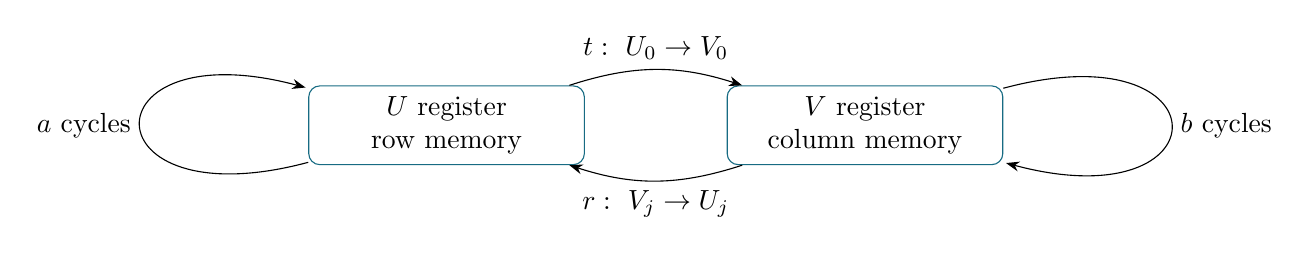
\begin{tikzpicture}[>=Stealth,node distance=15mm,
  state/.style={draw=accent,rounded corners,minimum width=35mm,
    minimum height=10mm,align=center}]
\node[state] (U) {$U$ register\\row memory};
\node[state,right=18mm of U] (V) {$V$ register\\column memory};
\draw[->] (U) edge[bend left=18] node[above] {$t:\ U_0\to V_0$} (V);
\draw[->] (V) edge[bend left=18] node[below] {$r:\ V_j\to U_j$} (U);
\draw[->] (U) edge[loop left] node[left] {$a$ cycles} (U);
\draw[->] (V) edge[loop right] node[right] {$b$ cycles} (V);
\end{tikzpicture}
\caption{The four fixed relations. Identity edges of $a,b,t$ are
specified in \eqref{comp:a}--\eqref{comp:t}. The final $r$ has no
edge out of $U$, forcing exactly one successful crossing per block.}
\label{comp:register-figure}
\end{figure}

\begin{corollary}[Concatenations and multiplicity]\label{comp:products}
On the boundary states $U$, the relation of
$w(R_1)\cdots w(R_\ell)$ is exactly the Boolean product
$R_1\cdots R_\ell$. More strongly, its matrix of numbers of paths
between $U$ states is the ordinary nonnegative-integer matrix product
of the zero-one matrices of the $R_i$.
\end{corollary}

\begin{proof}
Theorem~\ref{comp:register} identifies each single-block path-count
matrix on $U$ with the corresponding zero-one matrix. Every
surviving path is in $U$ at each block boundary, so concatenation
uses the usual sum over intermediate states. The empty
concatenation gives the identity matrix. Taking the support of
the integer product gives the Boolean product.
\end{proof}

The exact path-count statement is stronger than the language
equivalence needed below. It provides a useful independent test:
spurious duplicate branches cannot hide behind Boolean
reachability. It also makes clear that the full NFA need not be
unambiguous. Concatenations can have several intermediate-state
paths between the same endpoints.

\subsection{A complete binary language with \texorpdfstring{$6h+2$}{6h+2} states}
\label{comp:binary}

Use the fixed code
\begin{equation}\label{comp:bit-code}
 a\mapsto00,\qquad b\mapsto01,\qquad
 t\mapsto10,\qquad r\mapsto11,
\end{equation}
and let $\enc(R)=\code(w(R))$.
For each $q\in U\cup V$ take three decoder states
\[
 (q,\eps),\quad(q,0),\quad(q,1).
\]
From $(q,\eps)$ the first bit $d$ goes to $(q,d)$; from $(q,d)$
the second bit $e$ executes the four-letter relation corresponding
to $de$ and returns to a boundary state $(q',\eps)$.
All these transitions move right.

Add one initial state $q_{\mathrm{in}}$ and one accepting state
$q_{\mathrm{acc}}$. On $\Lmark$, $q_{\mathrm{in}}$ guesses any
$(U_i,\eps)$ and moves right. At $\Rmark$, each $(U_i,\eps)$
has a stay move to $q_{\mathrm{acc}}$. All other endmarker
transitions are undefined, and $q_{\mathrm{acc}}$ has no successors.
No other state is accepting.

This specifies a language $B_h$ on \emph{every} binary string.
An odd-length string ends in a pending-bit state and rejects.
An even-length string is decoded in consecutive two-bit groups;
it accepts precisely when some resulting four-letter path starts
and ends in $U$. There is no promise that the word consists of
canonical relation blocks and no unstated treatment of malformed
blocks. Some noncanonical even-length words may accept, according
to this explicit transition table. The empty binary word accepts.

\begin{proposition}[Binary state and length counts]\label{comp:binary-count}
The specified automaton is a $6h+2$-state 1NFA and, for every
finite sequence of $h$-point relations,
\begin{equation}\label{comp:canonical-membership}
 \enc(R_1)\cdots\enc(R_\ell)\in B_h
 \quad\Longleftrightarrow\quad R_1\cdots R_\ell\ne0.
\end{equation}
The canonical block length is
\[
 |\enc(R)|=2(h^2+h+1+|R|)\le4h^2+2h+2.
\]
\end{proposition}

\begin{proof}
There are $2h$ relation states with three decoder copies each,
plus the two explicitly added states. The decoder executes exactly
one four-letter transition per two input bits. On a canonical
concatenation, Corollary~\ref{comp:products} gives precisely the
relation product on the $U$ boundary states. The initial and final
rules test whether this relation has any pair. This includes
$\ell=0$, since $\Id_U$ is nonempty. The length formula follows
from Theorem~\ref{comp:register}.
\end{proof}

The order of the block length cannot be improved for an injective
binary encoding of all relations. There are $2^{h^2}$ distinct
relations, but only $2^{L+1}-1$ binary strings of length at most $L$.
Thus the largest block length of any such encoding is at least
$h^2$. In this sense the quadratic maximum length is optimal up
to a constant factor. This counting observation does not imply
optimality of the number of compiler states.

\subsection{Singleton contexts force the full relation divisor}
\label{comp:quotient-section}

Let $\eta:\bits^*\to M$ be a monoid homomorphism into any monoid
which recognizes $B_h$: assume there is a set $A\subseteq M$ such
that $w\in B_h$ exactly when $\eta(w)\in A$. This includes
recognition by ordinary-symbol matching diagrams, since the two
endmarker diagrams and the test ports define the set $A$.

Let $S\subseteq M$ be the submonoid generated by
$\{\eta(\enc(R)):R\in\Rel{[h]}\}$. It contains the empty product,
with the same identity as $M$. We only require a relation quotient
on $S$, not on all of $M$.

\begin{lemma}[Encoded context separation]\label{comp:quotient}
There is a well-defined unital surjective homomorphism
\[
 \phi:S\twoheadrightarrow\Rel{[h]},\qquad
 \eta(\enc(R_1)\cdots\enc(R_\ell))
       \longmapsto R_1\cdots R_\ell .
\]
\end{lemma}

\begin{proof}
Suppose two canonical concatenations have the same element of
$M$, but their relation products $R$ and $T$ differ. Choose
$(i,j)$ in their symmetric difference and put
$E_i=\{(i,i)\}$ and $E_j=\{(j,j)\}$. Then
\[
 E_i R E_j\ne0\quad\Longleftrightarrow\quad(i,j)\in R,
\]
and the corresponding equivalence holds for $T$.
Surround each canonical concatenation by $\enc(E_i)$ on the left
and $\enc(E_j)$ on the right. By
\eqref{comp:canonical-membership}, precisely one resulting binary
word belongs to $B_h$. Yet multiplicativity of $\eta$ makes their
images equal, contradicting recognition. This proves
well-definedness, including comparisons with an empty
concatenation.

Concatenating representatives proves multiplicativity. The empty
word is sent to $\Id_{[h]}$, so the map is unital. Every relation
is the image of its single canonical block, proving surjectivity.
\end{proof}

This is the usual singleton-context syntactic argument, specialized
to the encoded submonoid; compare
\cite{Pin1997,OpenAILiveness2026}. A decoder need not label every
arbitrary binary word by an $h$-point relation in a multiplicative
way. The narrower generated submonoid is both sufficient and
necessary for the argument as stated.

\subsection{Proof and quantitative comparison}
\label{comp:main-proof}

\begin{proof}[Proof of Theorem~\ref{intro:main}]
Take the binary language from Proposition~\ref{comp:binary-count}
and an equivalent $s$-state 2DFA. By
Theorem~\ref{mach:representation}, its ordinary-symbol matching
diagrams lie in $\Br{k}$ for some $k\le8s+2$ and recognize $B_h$
with fixed endmarker diagrams and fixed test ports.
Lemma~\ref{comp:quotient} supplies an identity-containing
submonoid with a unital surjection onto $\Rel{[h]}$.
Theorem~\ref{alg:divisor} therefore gives
$8s+2\ge k\ge F(h)$, proving \eqref{intro:h-bound}.

For $n\ge14$, put $h=\lfloor(n-2)/6\rfloor\ge2$. The source has
$6h+2\le n$ states and may be padded with unreachable,
nonaccepting states to reach exactly $n$. Integer floor
arithmetic gives
\[
 \left\lfloor\frac{\lfloor(n-2)/6\rfloor-2}{9}\right\rfloor
 =\left\lfloor\frac{n-14}{54}\right\rfloor.
\]
Solving \eqref{intro:h-bound} for $s$ proves
\eqref{intro:n-bound}. The exponential asymptotic follows by
absorbing the floor and fixed multiplicative factors into $O(1)$.
\end{proof}

The integer recurrence of Proposition~\ref{alg:finite-recurrence}
gives the useful finite refinement
\begin{equation}\label{comp:integer-bound}
 s\ge
 \max\left\{1,\left\lceil\frac{D(h)-1}{4}\right\rceil\right\}.
\end{equation}
The additional $1$ simply records that a recognizer has at least
one state. The supplied recurrence script computes $D(h)$
using exact integers; no floating-point rounding enters
\eqref{comp:integer-bound}.

\begin{table}[tb]
\centering
\small
\begin{tabular}{p{0.26\textwidth}p{0.31\textwidth}p{0.31\textwidth}}
\toprule
Quantity & Inspected earlier construction & This article\\
\midrule
Relation-divisor degree
& $2^{\lfloor(h-2)/31\rfloor}$
& $2(5/2)^{\lfloor(h-2)/9\rfloor}$\\[3pt]
2DFA matching degree
& $4(s+1)^2$ for arbitrary alphabets
& $2(a+2)s+2$ for $a$ letters\\[3pt]
Binary matching degree
& general bound $4(s+1)^2$
& $8s+2$\\[3pt]
Four-letter relation compiler
& $3h$ states in R816's convention
& $2h$ relation states\\[3pt]
Binary source count
& $9h$ states in R816's convention
& $6h+2$ including our marker states\\[3pt]
Binary conclusion
& constant-factor transfer applies to an imported liveness bound
& explicit bound \eqref{intro:n-bound}\\
\bottomrule
\end{tabular}
\caption{Comparison with the source matching argument
\cite{OpenAILiveness2026} and the earlier encoding record
\cite{TheoremDBR816}. Machine conventions explain the two added
marker states in the present source count. The general quadratic
port bound can be preferable when the alphabet is very large.}
\label{comp:comparison}
\end{table}

The leading exponential rate in the algebraic degree estimate
increases from $1/31$ to $\log_2(5/2)/9$ when measured in $h$.
The sparse matching representation then avoids taking a square
root of that degree lower bound for a fixed alphabet. These
are separate improvements; the binary encoding permits both
to contribute to a bound measured in the number of source
states. The lower bound concerns states, not running time,
number of head reversals, or the length of a transition-table
description.

\section{A separate consequence for binary complementation}
\label{complement:section}

The binary compiler also transfers an exponential lower bound when
the machine recognizing the complementary language may itself be
nondeterministic. This section uses one external algebraic theorem
from \cite{OpenAIComplement2026}, identified below. The determinization
theorem proved earlier is independent of this imported premise.

\subsection{The external path-diagram bound}

For $m\ge1$, take disjoint sets $D^+,D^-$, each with $m$ labels.
A path diagram is a quadruple of relations
\[
 F\subseteq D^+\times D^+,\quad
 B\subseteq D^-\times D^-,\quad
 L\subseteq D^+\times D^-,\quad
 R\subseteq D^-\times D^+.
\]
The positive sign denotes entry from the left and the negative sign
entry from the right. The relations $F,B$ describe through paths;
$L,R$ describe returns to the side of entry. Product means joining
adjacent boundaries and recording finite paths from an outer entry
to the first outer exit. Expanding and contracting traversals of a
consecutive block proves associativity. The identity has identity
through relations and empty return relations. Write $\mathcal T_m$
for this finite monoid and $z\sqsubseteq w$ for inclusion in all four
relations. Multiplication preserves $\sqsubseteq$ in both arguments.

\begin{center}
\fbox{\begin{minipage}{0.92\linewidth}
\begin{theorem}[Imported order-reversing image bound]
\label{complement:imported}
Let $m\ge1$, let $H$ be a finite set with $h\ge2$ elements, and let
$S_0$ be a submonoid of $\mathcal T_m$. Suppose a surjective
multiplicative map $\phi_0:S_0\to\Rel{H}$ satisfies
\[
 z\sqsubseteq w\quad\Longrightarrow\quad
 \phi_0(w)\subseteq\phi_0(z)
 \qquad(z,w\in S_0).
\]
Then
\begin{equation}\label{complement:external-bound}
 2m\ge2^{\lfloor(h-2)/127\rfloor}.
\end{equation}
Identity preservation of $\phi_0$ is not required.
\end{theorem}
This is the theorem entitled \emph{Order-reversing image bound},
source label \texttt{amp:image}, in Section~2 of
\cite{OpenAIComplement2026}. Its full hypotheses and numerical
conclusion are stated here; its proof by missing recurrent classes
and nested corners is not reproduced in this article.
\end{minipage}}
\end{center}

The parameter $m$ counts labels in each direction. Thus the quantity
in \eqref{complement:external-bound} is the total number $2m$ of
directional labels; it is not the degree of the Brauer matching
representation used in the determinization proof.

\begin{lemma}[Finite acceptance and monotonicity]
\label{complement:representation}
For an $s$-state binary 2NFA $C$ in the endmarker model of this article,
there are a homomorphism $\tau:\bits^*\to\mathcal T_{s+1}$,
fixed endmarker diagrams $\lambda,\rho$, and positive labels $a,b$
such that
\begin{equation}\label{complement:acceptance}
 u\in L(C)\quad\Longleftrightarrow\quad
 (a,b)\in F_{\lambda\tau(u)\rho}.
\end{equation}
Consequently $\tau(u)\sqsubseteq\tau(v)$ implies
\begin{equation}\label{complement:monotonicity}
 xuy\in L(C)\quad\Longrightarrow\quad xvy\in L(C)
 \qquad(x,y\in\bits^*).
\end{equation}
\end{lemma}

\begin{proof}
The finite-computation construction of \cite{OpenAIComplement2026}
has the following exact normalization. Add one new success state.
From every original accepting state, allow a stay move into it; in
the new state sweep right and make one designated artificial exit
past the right endmarker. This exit represents acceptance and is
not an additional move available to the original machine. A finite
computation reaches it precisely when an original finite computation
has reached an accepting state, including an accepting initial state.

Use the resulting $s+1$ states as labels in each direction. For each
cell symbol, including markers, a local diagram edge records any
finite sequence of stay transitions followed by one exit move from
the cell. The entry sign records the side of arrival. Finite
computations split into such visits, and local edge witnesses
concatenate back into finite computations. This gives
\eqref{complement:acceptance} with the marker diagrams fixed and
the ordinary-cell products defining $\tau$. Missing transitions and
infinite nonaccepting computations create no finite successful path.
Finally, inclusion of all four relations is preserved by adjoining
the diagrams for $x,y$ and the markers. The designated accepting
edge therefore persists, proving \eqref{complement:monotonicity}.
\end{proof}

\subsection{Encoded contexts give the required antitone quotient}

Let $H=[h]$ and let $B_h$ be the binary language constructed above,
recognized by a $6h+2$-state 1NFA. For a word $w=R_1\cdots R_t$ over the formal
alphabet $\Rel{H}$, write
\[
 r(w)=R_1\cdots R_t,\qquad
 \enc(w)=\enc(R_1)\cdots\enc(R_t),
\]
and use $r(\eps)=\Id_H$, $\enc(\eps)=\eps$. The compiler proves
\begin{equation}\label{complement:compiler-property}
 \enc(w)\in B_h\quad\Longleftrightarrow\quad r(w)\ne\varnothing.
\end{equation}
The transition tables also define $B_h$ on every other binary word,
so complementation below is taken in the full set $\bits^*$.

\begin{proposition}[Direct antitone quotient]\label{complement:quotient}
If an $s$-state 2NFA $C$ recognizes $\bits^*\setminus B_h$, a
submonoid of $\mathcal T_{s+1}$ admits a surjective unital
homomorphism onto $\Rel{H}$ that reverses inclusion.
\end{proposition}

\begin{proof}
Use $\tau$ from Lemma~\ref{complement:representation} and let
\[
 S_0=\{\tau(\enc(w)):w\in\Rel{H}^{*}\}.
\]
This is the submonoid generated by the diagrams of the individual
encoded relations, including the empty product. Suppose
$\tau(\enc(u))\sqsubseteq\tau(\enc(v))$.
Fix $i,j\in H$ and use the binary contexts
$x=\enc(\Id_{\{i\}})$ and $y=\enc(\Id_{\{j\}})$.
For every relation $A$, the product $\Id_{\{i\}}A\Id_{\{j\}}$
is empty exactly when $(i,j)\notin A$. Hence
\eqref{complement:compiler-property}, followed by complement
acceptance and \eqref{complement:monotonicity}, gives
\[
 (i,j)\notin r(u)\quad\Longrightarrow\quad(i,j)\notin r(v).
\]
Thus $r(v)\subseteq r(u)$. Equality of the two diagrams gives this
inclusion in both directions, so
\[
 \phi_0\bigl(\tau(\enc(w))\bigr)=r(w)
\]
is well-defined. Concatenation proves multiplicativity, the empty
word proves unitality, and every $A\in\Rel{H}$ is the image of
$\tau(\enc(A))$. The implication just proved is the required
order reversal.
\end{proof}

\begin{theorem}[Binary nondeterministic complementation]
\label{complement:binary}
Under the imported premise of Theorem~\ref{complement:imported},
every $s$-state 2NFA recognizing $\bits^*\setminus B_h$ satisfies
\begin{equation}\label{complement:state-bound}
 2(s+1)\ge2^{\lfloor(h-2)/127\rfloor},\qquad
 s\ge\frac12\,2^{\lfloor(h-2)/127\rfloor}-1.
\end{equation}
Consequently, for each $n\ge14$, an $n$-state binary one-way NFA has
a complementary language requiring at least
\begin{equation}\label{complement:n-bound}
 \frac12\,2^{\lfloor(n-14)/762\rfloor}-1
\end{equation}
states in every two-way nondeterministic recognizer.
\end{theorem}

\begin{proof}
Apply Theorem~\ref{complement:imported} to
Proposition~\ref{complement:quotient}, with $m=s+1$.
For the last assertion choose $h=\lfloor(n-2)/6\rfloor$ and add
unreachable states to $B_h$ to obtain exactly $n$ states.
The identity
$\lfloor(h-2)/127\rfloor=\lfloor(n-14)/762\rfloor$
gives \eqref{complement:n-bound}.
\end{proof}

The same homomorphism $\tau$ and its $2(s+1)$ directional labels are
used throughout this argument. In particular, encoded word length
does not introduce a state factor. The external dependency is
specifically Theorem~\ref{complement:imported}; the encoding and
the antitone-quotient argument have been given here. This article
provides no new Lean formalization of that imported theorem or of
this complementation transfer. The compiler's finite exact audits
verify its stated encoding behavior and do not certify the external
path-diagram bound.

\section{Exact finite audits and reproducibility}
\label{verify:section}

The universal claims in this article are proved mathematically.
The accompanying programs test independent representations of the
objects involved, with special attention to failure modes that are
easy to miss in a diagram argument: reversed product conventions,
loops and parallel edges, pending binary bits, multiplicity of
paths, and spurious dependence on an adjacent input symbol.
These computations support the implementation and exposition.
They are not finite substitutes for the induction, a proof-assistant
formalization, or a certificate of bibliographic novelty.

\subsection{Idempotent structure}

The script \texttt{code/brauer\_audit.py} enumerates every perfect
matching on $2m$ ports for $0\le m\le7$, a total of 146,600
diagrams. Its primary test of idempotence computes the literal
three-layer graph product $e^2$ and compares the resulting matching
with $e$. A separate graph predicate tests the alternating-component
classification. The enumeration includes nonidempotents, so the
classification is not used to generate only purported positive
examples.

For the idempotents it checks the sharp support bound, the exact
deficit identity, equality structure, fixed-rank maxima, the
component-deletion stability statement, and the maximizer count.
The observed totals are:
\begin{center}
\begin{tabular}{rrrr}
\toprule
$m$ & All diagrams & Idempotents & Support equality cases\\
\midrule
0 & 1 & 1 & 1\\
1 & 1 & 1 & 1\\
2 & 3 & 2 & 1\\
3 & 15 & 10 & 7\\
4 & 105 & 40 & 25\\
5 & 945 & 296 & 61\\
6 & 10,395 & 1,936 & 481\\
7 & 135,135 & 17,872 & 2,731\\
\bottomrule
\end{tabular}
\end{center}
An equality case here means $|\supp(e)|=3\crk(e)/2$,
including the identity. The counts do not assert that every
fixed-rank support maximizer must attain that equality when
$m<3\crk(e)/2$.

\subsection{The repetition-independent budget}

The script \texttt{code/idempotent\_budget\_audit.py} uses literal
diagram multiplication from the preceding script. For every
ordered idempotent pair through degree four, it tests the relative
corner bound along all positive powers up to the first repetition.
It also closes each pair of distinct idempotent generators under
multiplication and checks every resulting element. The exact
coverage is 1,706 ordered corner pairs, 1,898 distinct positive
corner powers, and 826 complete generated monoids containing
4,280 inspected elements when counted separately for each
generating family.

The same program samples reproducible families in degrees zero
through twelve, with the seed recorded in its JSON output. It
tests 3,250 corner pairs, 3,250 families of two to four
idempotents, 195,000 repeated-word prefixes, and 3,442
final-word powers. Each family also receives a graph check of
component invariance, even cap-edge counts, and the identity
between the total edge budget and the sum of generator coranks.
These larger-degree checks are sampled, and are labeled as such.

\subsection{The relation compiler}

The script \texttt{code/relation\_compiler\_audit.py} independently
constructs the four-letter transition tables and the binary decoder.
It compares path counts using arbitrary-precision nonnegative
integers, not just Boolean reachability.

\begin{center}
\begin{tabular}{p{0.65\textwidth}r}
\toprule
Test family & Cases\\
\midrule
Every individual relation for $1\le h\le4$ & 66,066\\
Every ordered pair of relations for $1\le h\le3$ & 262,404\\
Singleton entry tests for every relation, $1\le h\le3$ & 4,674\\
Every binary string of length at most twelve, $1\le h\le4$ & 32,764\\
\midrule
Total & 365,908\\
\bottomrule
\end{tabular}
\end{center}
The arbitrary-string tests include odd lengths and noncanonical
even words. They compare the actual pending-bit behavior with
direct decoding. For canonical concatenations, the expected
path-count matrix is an ordinary integer matrix product,
so accidental duplicate paths are detectable.

\subsection{Actual symbol-local matching diagrams}

The script \texttt{code/sparse\_slots\_audit.py} constructs the
local lane graphs themselves, contracts them to perfect matchings,
multiplies those matchings, and compares the test-port predicate
with direct execution of the original deterministic machine.
It does not infer the result by applying a graph-connectivity
predicate to an already assembled whole-input graph.

Every legal one-state binary machine in the stated model is
tested: there are 288, including both choices of accepting set
and all legal partial transition rows at the two ordinary symbols
and two markers. An additional 512 two-state machines are sampled
with a fixed seed. Each is tested on all 63 binary words of
length at most five. The audit constructs 3,200 local diagrams
and performs 50,400 machine-word comparisons.

The direct executions include 24,066 initial acceptances, 4,367
later acceptances, 12,637 rejecting infinite runs, and 9,330
undefined rejecting halts. Every local matching is checked to
be perfect and to satisfy $k\le8s+2$. This explicitly exercises
the corner cases in Section~\ref{mach:section}.

\subsection{Exact recurrence and finite consequences}

The script \texttt{code/finite\_bounds.py} evaluates
\eqref{alg:D} through $h=256$, using only integer ceilings.
It also verifies the explicit union-graph obstruction in
Section~\ref{research:union}. Selected values are:
\begin{center}
\small
\begin{tabular}{rrrrr}
\toprule
$h$ & Source states $6h+2$ & $\lceil F(h)\rceil$
 & Degree bound $2D(h)$ & 2DFA states, at least\\
\midrule
10 & 62 & 2 & 6 & 1\\
20 & 122 & 13 & 18 & 2\\
50 & 302 & 196 & 416 & 52\\
100 & 602 & 19,074 & 66,452 & 8,307\\
200 & 1,202 & 1,136,868,378 & 1,769,699,850 & 221,212,481\\
\bottomrule
\end{tabular}
\end{center}
The last column applies \eqref{comp:integer-bound} to the exact
recurrence. The closed form remains useful because it gives a
simple exponential statement for all parameters; the recurrence
preserves the improvements from parity and the best arm sizes
at each finite stage.

\subsection{Reproduction and interpretation}

From the extracted package directory, run:
\begin{verbatim}
python3 code/run_all.py --output-dir reproduced
\end{verbatim}
All audit programs require only Python's standard library.
The runner invokes them with Python optimization enabled;
mathematical checks raise explicit exceptions rather than relying
on removable assertion statements. The \texttt{certificates}
directory contains the executed reference outputs, including the
random seeds, parameter ranges, and a case-stream digest for the
relation compiler. Timing fields and local output paths may
change across runs; mathematical counts and the fixed case-stream
digest should agree.

The article can be rebuilt with the supplied Makefile, using
\texttt{pdflatex} and \texttt{bibtex}. TeX source, bibliography,
audit programs, reference JSON, exact recurrence CSV, source
provenance, theorem ledger, and licensing notices are supplied
together. No remote network access is required for compilation
or for any mathematical audit.

The independent review performed during preparation checked
the algebraic corners, the amplifier, the modular compiler,
the machine convention, and the sparse local construction.
It was an additional AI-assisted mathematical review, not
independent human peer review. The source snapshots and precise
theorem dependencies make subsequent human or formal review
possible without reconstructing the research session.

\section{Further research: precise questions and useful obstructions}
\label{btc:research:section}

The results settle several quantitative issues within the
matching-monoid approach, but leave substantial structural problems.
The following questions are chosen so that a successful answer
would improve a theorem, identify a genuine barrier, or produce
a reusable formal component.

\subsection{The true degree of a full relation divisor}

Let $\beta(h)$ be the least $m$ for which an identity-containing
submonoid of $\Br{m}$ admits a unital surjection onto $\Rel{[h]}$.
Existence follows from the constructions in this article, and
its growth is already pinned down to exponential order.
That order already follows from the earlier exponential source
bound and its general machine representation
\cite{OpenAILiveness2026}; the following consequence records
explicit bounds from the constructions given here.

\begin{proposition}\label{btc:research:beta}
For $h\ge2$,
\begin{equation}\label{btc:research:beta-bounds}
 2(5/2)^{\lfloor(h-2)/9\rfloor}
 \ \le\ \beta(h)\ \le\ 12\cdot4^h+26.
\end{equation}
In particular $\beta(h)=2^{\Theta(h)}$.
\end{proposition}

\begin{proof}
The lower bound is Theorem~\ref{btc:alg:divisor}.
Consider the four-letter language defined by starting with any
state in $U$ and accepting at the end exactly in $U$, using
\eqref{btc:comp:a}--\eqref{btc:comp:r}. A deterministic subset machine
has at most $2^{2h}$ subset states, one separate initial state,
and one separate accepting state. On the left marker it enters
the subset $U$; on each ordinary symbol it takes the relational
image of its current subset; on the right marker it enters the
accepting state exactly when its subset meets $U$. All subset
states are nonaccepting, so this respects the convention of
Section~\ref{btc:intro:model}.

For $a=4$, Theorem~\ref{btc:mach:representation} gives degree at most
$12(2^{2h}+2)+2$. Canonical four-letter words and their singleton
contexts give the surjection by the same proof as
Lemma~\ref{btc:comp:quotient}, before binary decoding.
This is the claimed upper bound.
\end{proof}

\begin{question}
What are the exponential rate and leading corrections of $\beta(h)$?
Does $\lim_{h\to\infty}h^{-1}\log_2\beta(h)$ exist?
Can one construct a significantly smaller matching representation
of the full relation monoid, or prove a stronger divisor obstruction?
\end{question}

The current proof yields a lower rate $\log_2(5/2)/9$ and an
upper rate $2$. Establishing a suitable product, submultiplicative,
or supermultiplicative relation for $\beta$ could first settle
existence of a rate. A direct representation may improve the
upper bound more effectively than determinizing the compiler.

\subsection{Beyond rectangular relation addition}

\begin{question}
Can a nonrectangular family of relation additions improve the
gain-to-deletion ratio of Proposition~\ref{btc:alg:amplification}?
\end{question}

The $p\times q$ grid adds $pq$ independent edges at a cost of
$p+q$ conjugates and deletes $p+q-1$ points when isolating one
addition. The choice $(5,5)$ is optimal only for this architecture.
A better construction needs a different incidence pattern,
a way to share witnesses without leaving earlier edges in the
retained corner, or a stronger simultaneous local lower bound.
Optimizing $p,q$ again cannot improve the fixed-parameter rate
already proved.

One concrete starting point is a directed acyclic incidence
system with several intermediate vertices. Its products must
be tracked exactly: accidental length-two paths may add
unwanted relations and destroy the singleton-corner property.
An optimization problem based only on edge counts would miss
this obstruction.

\subsection{Minimum generated rank needs more than union connectivity}
\label{btc:research:union}

The budget theorem uses a union graph and parity. Those data
need not determine the actual minimum rank in the generated
monoid.

\begin{proposition}[A connected union need not attain its parity floor]
\label{btc:research:union-obstruction}
There are two rank-two idempotents in $\Br{4}$ whose union cap
graph is connected, although every nonempty word in them has
rank two.
\end{proposition}

\begin{proof}
Use labels $0,1,2,3$. Let $a$ have left cap $\{0,1\}$, right
cap $\{1,2\}$, and transversals $2\to0$, $3\to3$.
Let $b$ have left cap $\{0,1\}$, right cap $\{1,3\}$, and
transversals $3\to0$, $2\to2$. Each consists of one
three-vertex alternating path and one fixed point, so each is
idempotent of rank two.

Direct gluing gives $ab=b$ and $ba=a$; the left caps agree,
and tracing each of the two remaining transversal paths
gives the stated right factor. Thus every nonempty word
equals its last letter, and the generated monoid is
$\{\Id,a,b\}$.
The union cap graph has edges $\{0,1\}$, $\{1,2\}$, and
$\{1,3\}$, with the first edge occurring twice. It is connected
on four vertices, for which the component parity lower bound
on rank is zero. That value is not attained.
\end{proof}

\begin{question}
Which additional data determine the minimum rank of a monoid
generated by Brauer idempotents, or characterize equality in
the corank budget?
\end{question}

Generator identities, cap colors, and how alternating
connectors interact matter beyond uncolored connectivity.
A promising formulation is to retain each generator's
two colored matchings on each invariant component and study
the semigroup of induced endpoint connectors. A useful
theorem would characterize the existence of a word attaining
the component parity floor, with an effective bound on the
length of a witnessing word.

\subsection{Optimal compiler size and ambiguity}

\begin{question}
What is the least asymptotic number of states needed by a
fixed-alphabet NFA compiler whose canonical words realize
every relation on $h$ designated boundary states?
\end{question}

Our four-letter compiler uses $2h$ relation states and a
binary decoder with $6h+2$ total states in the stated model.
The block length is optimal in order by counting, but that
argument does not bound compiler states beyond the designated
boundary requirement. A smaller binary construction would
improve the coefficient in \eqref{btc:intro:n-bound} without
changing the algebra.

The strong single-block path-count property suggests a
related question: can the same state order and block length
be retained under a useful bound on ambiguity across
concatenations? Single-block uniqueness alone is insufficient;
ordinary matrix multiplication already records potentially
many intermediate paths. Results for globally unambiguous
sources require a new construction or a structural obstruction.

\subsection{The constant in sparse matching representations}

\begin{question}
Can every binary $s$-state 2DFA be represented in Brauer
degree $cs+O(1)$ for a constant $c<8$, and what is the best
universal constant?
\end{question}

Theorem~\ref{btc:mach:linear-optimality} rules out sublinear
degree, but leaves a gap in the coefficient. The present
construction uses two lanes for every distinct crossing triple.
Several transitions may share a port scheme if they cannot
conflict in any local symbol diagram. Any proposed reuse must
preserve target-side locality and distinguish all possible
arrivals; looking only at transitions active in one completed
input word is not sufficient.

A sharper machine-specific invariant than the number of
candidate triples may be a useful first target. For example,
one can ask for the minimum number of compatible slot classes
under simultaneous local matching constraints, then compare
that combinatorial optimum with the number of states.

\subsection{Ordered path monoids and nondeterministic complement}

\begin{question}
Is there a repetition-independent structural budget for
idempotents in the ordered path-diagram monoid used in
Section~\ref{btc:complement:section}?
\end{question}

The Brauer proof relies on degree-two colored components
and a parity restriction on rank. General path relations
branch, so those arguments do not transfer directly.
Nevertheless, an invariant controlling the loss of
recurrent classes through many repeated idempotents could
replace the analogous losses in the imported
complementation amplifier. This is a specific route to
improving the constant $127$, with an explicit reason why
the present theorem does not already do so.

\subsection{Uniformity and short witnesses}

\begin{question}
What quantitative length bound can be put on a binary word
distinguishing a small candidate 2DFA from $B_h$, as a
function of $h$ and the candidate's number of states?
\end{question}

The encoding of one relation has length $O(h^2)$, but the
semigroup proof may take long words and idempotent powers.
An exponential state obstruction is therefore not automatically
a useful short-input or time lower bound. Bounding the
necessary powers and context lengths could illuminate the
connection with resource-bounded uniform simulation.
Any proposed implication for logarithmic space must explicitly
account for constructibility and the relation between witness
length and source description size.

\subsection{A practical formalization program}

\begin{question}
Can the new corank budget and sparse representation be
formalized as independent reusable modules, then combined
with the existing liveness formalization?
\end{question}

The natural first module represents Brauer multiplication
by perfect matchings and finite graph connectivity, proves
the colored-component classification, and derives the budget.
The second module proves the corner reduction and the
minimum-rank unit-lifting lemma in a reusable finite-semigroup
interface. The third gives the $p,q$ amplification with
ambient ranks and relative coranks distinguished in the types.
These algebraic modules should be completed before encoding
the entire automaton construction.

On the machine side, finite successor graphs and a precise
cycle of directed tree edges provide a tractable interface.
The local lane graph should be defined once and related both
to Brauer multiplication and to the configuration semantics.
The existing exact programs can produce regression examples,
but a kernel proof must establish the universal correspondence.
A final arithmetic layer can prove the decoder counts, floor
identities, and the closed recurrence. This order isolates
the two most consequential mathematical risks: faithful
corner reduction and symbol locality.

\subsection{Research priorities}

For immediate continuation, the most focused tasks are:
formalize the short corank-budget proof; characterize when
the generated minimum rank attains the union-component
parity bound; and search for a smaller direct binary compiler.
Each has a compact mathematical specification and a clear
effect on the present results. The longer-term target is
the exact exponential behavior of $\beta(h)$, together
with a stronger ordered-path invariant for complementation.

\begin{writenote}[Under Vladimir's standing rule of 4 October 2026, 7 October 2026]
The eight research questions stand as the source states them, and none is
answered elsewhere in the repository. The write found no claim of the source
that is unproved as stated outside them, and none that is wrong; nothing was
moved here or refuted. Theorem~\ref{btc:complement:binary} is not an
unproved claim in this sense, because the source states it as conditional on
a named external premise; it stays where it is, marked conditional
(Section~\ref{btc:complement:section}). Proposition~\ref{btc:research:beta}
was rederived ($12(2^{2h}+2)+2=12\cdot4^h+26$; the subset machine accepts
only through its separate accepting state), and
Proposition~\ref{btc:research:union-obstruction} was confirmed by the write's
own diagram multiplication ($a,b$ idempotent of rank two, $ab=b$, $ba=a$).
\end{writenote}
\begin{writenote}[Independent check of the write, 9 October 2026]
An adversarial check made by the intake after the write (commit
\file{d89be4d77}) re-derived the statements marked [write] with its own code.
\emph{The headline bound}, checked the hardest: the chain
Theorem~\ref{btc:alg:rank} (base $2\le h\le10$, step $h\ge11=p+q+1$ with
$(5/2)F(h-9)=F(h)$), Theorem~\ref{btc:alg:divisor},
Theorem~\ref{btc:mach:representation} ($J\le4s+1$ for $a=2$),
Lemma~\ref{btc:comp:quotient} and the proof in
Section~\ref{btc:comp:main-proof} was re-derived, with the floor identities
$\lfloor(\lfloor(n-2)/6\rfloor-2)/9\rfloor=\lfloor(n-14)/54\rfloor$ and the
analogue for $127$ and $762$ checked for $14\le n<10^6$. The sparse-slot
representation, read but not rebuilt at the write and at intake, was rebuilt
by the check from the text of Section~\ref{btc:mach:section} alone (sink
normalization, candidate set, asymmetric attachment with fresh leaves, the
two test edges, two lanes per edge, rotation joins, contraction): on 400
random binary 2DFAs with $1\le s\le4$ states and all $127$ binary words of
length at most $6$, the test-port predicate agreed with direct execution in
all $50{,}800$ comparisons (both test ports matched whenever one was), and
always $k\le8s+2$; a deliberately broken attachment rule produced $1{,}482$
mismatches in a smaller run, so the comparison discriminates. The compiler
path counts of Theorem~\ref{btc:comp:register} and
Corollary~\ref{btc:comp:products} (every relation for $h\le3$ and every
ordered pair for $h\le2$; random relations and pairs for $h=3,4$) and the
binary decoder's
membership \eqref{btc:comp:canonical-membership} on $4{,}500$ canonical
concatenations were recomputed by an own simulation, with no mismatch.
\emph{The recurrence}: $D(h)$ recomputed with exact rational ceilings for
$h\le256$ equals every one of the 255 rows of
\file{certificates/finite\_bounds.csv} in all columns (source states, the
old bound $2^{\lfloor(h-2)/31\rfloor}$, $\lceil F(h)\rceil$, $D$, $2D$, the
state bound $\max\{1,\lceil(D-1)/4\rceil\}$), each recorded arm sum is a
maximizer, $2D(h)\ge\lceil F(h)\rceil$ throughout, and the five table rows
of Section~\ref{btc:verify:section} agree. \emph{Status of
Theorem~\ref{btc:complement:binary}}: nowhere in the article, the README or
the ledger is it presented as proved (the ledger: ``Proved transfer
conditional on named external premise''); the premise was compared word for
word with the companion's source and located in its Section~2 (precision at
the end of Section~\ref{btc:complement:section}). \emph{Labels}: with
\file{btc:} removed, every delivered line of the eight source files is
unchanged (317 lines inserted by the write); 91 delivered labels, 53
\verb|\ref| and 32 \verb|\eqref| references, all prefixed; one label added;
every delivered number unchanged against a build of the delivered text, and
the ledger's 20 numbers equal the delivered ones; the built bibliography
equals the delivered \file{article.bbl}. \emph{Other numbers}: own Brauer
multiplication for $m\le7$ (diagram, idempotent and support-equality counts
of the first table of Section~\ref{btc:verify:section}, no support-bound
violation); the shipped exhaustive counts $1{,}706$, $1{,}898$, $826$ and
$4{,}280$; the budget and the relative budget on $90{,}000$ random word
prefixes in idempotent powers of random diagrams, $3\le m\le10$, with no
violation; Proposition~\ref{btc:research:union-obstruction}; the rates (both
truncations), the optimum $(5,5)$ over $p,q\le300$, $312/343$, $5^7>2^{16}$,
$12(4^h+2)+2=12\cdot4^h+26$, and the case counts of
Section~\ref{btc:verify:section}. \emph{Provenance}: archive size, SHA-256, 32
files, 2{,}214 lines and 96{,}365 bytes, the 29 placed files byte-identical
(and unchanged since, except the files the write edited), the sizes of the
files not shipped and the 31 checksums, the author lines, the pin, the three
neighbour README blobs, and the absence of earlier repository files on
two-way automata or Brauer monoids confirmed. Apart from the two precisions
(the status note's list, and Lemma~\ref{btc:complement:representation}), no
defect was found in the write, and no claim of the source was found wrong.
\end{writenote}

\clearpage
\addcontentsline{toc}{section}{References}
\begingroup
\raggedright
\bibliographystyle{plain}
\bibliography{references}
\endgroup
\end{document}
